\documentclass[11pt,a4paper]{article}

\usepackage[margin=1in]{geometry}
\usepackage{amsmath,amssymb,amsthm,mathtools}
\usepackage{booktabs}
\usepackage{array}
\usepackage{enumitem}
\usepackage{xcolor}
\usepackage{tikz}
\usetikzlibrary{arrows.meta,positioning,calc,shapes.geometric}
\usepackage{microtype}
\usepackage[colorlinks=true,linkcolor=blue!60!black,citecolor=teal!70!black,urlcolor=blue!60!black]{hyperref}

% Theorem environments
\newtheorem{theorem}{Theorem}[section]
\newtheorem{lemma}[theorem]{Lemma}
\newtheorem{corollary}[theorem]{Corollary}
\newtheorem{proposition}[theorem]{Proposition}
\newtheorem{conjecture}[theorem]{Conjecture}
\newtheorem{claim}{Claim}[theorem]
\theoremstyle{definition}
\newtheorem{definition}[theorem]{Definition}
\newtheorem{remark}[theorem]{Remark}
\newtheorem{example}[theorem]{Example}

% Math macros
\newcommand{\mad}{\operatorname{mad}}
\newcommand{\ch}{\operatorname{ch}}
\newcommand{\N}{\mathbb{N}}
\newcommand{\Z}{\mathbb{Z}}
\newcommand{\Q}{\mathbb{Q}}
\newcommand{\R}{\mathbb{R}}
\newcommand{\Ppoor}{\mathcal{P}_1}
\newcommand{\code}[1]{\texttt{\detokenize{#1}}}

\title{Proper Conflict-Free $\kappa_G$-Choosability of Graphs with\\Maximum Average Degree Less Than $22/9$}

\author{
  Fanyi Wei\\[3pt]
  \small Harbin Institute of Technology\\[4pt]
  \small\textit{With complete machine-checked formal verification in Lean 4}
}

\date{\today}

\begin{document}
\maketitle

\begin{abstract}
A proper vertex coloring of a graph $G$ is \emph{proper conflict-free} (PCF) if every non-isolated vertex has at least one color appearing exactly once in its open neighborhood. Given a function $f : V(G) \to \N$, a graph $G$ is \emph{PCF $f$-choosable} if every list assignment $L$ with $|L(v)| \ge f(v)$ for all $v \in V(G)$ admits a PCF $L$-coloring. Kashima, \v{S}krekovski, and Xu recently introduced the tight degree-based threshold function
\[
  \kappa_G(v) = \begin{cases} 4, & \text{if } d_G(v) = 2,\\ d_G(v) + 1, & \text{if } d_G(v) \neq 2, \end{cases}
\]
and conjectured that every connected graph other than the $5$-cycle $C_5$ is PCF $\kappa_G$-choosable. Lu, Ying, and Song (2026) confirmed this conjecture for all connected graphs $G \not\cong C_5$ with $\mad(G) < 12/5$ (implying the result for planar graphs of girth at least $12$).

In this paper, we improve this threshold to $\mad(G) < 22/9$: every connected graph $G \not\cong C_5$ with $\mad(G) < 22/9$ is PCF $\kappa_G$-choosable. As an immediate consequence of Euler's formula, every planar graph of girth at least $11$ is PCF $\kappa_G$-choosable. Our proof introduces three main ingredients: (i)~a \emph{zero-auxiliary-graph core subgraph reduction} $K = G - X$ that eliminates the $r$-leaf-cycle auxiliary graph construction of Lu, Ying, and Song and applies uniformly to arbitrary rational density bounds; (ii)~an upgraded universal structural foundation valid for all $\mad(G) < 5/2$; and (iii)~five new families of reducible configurations---centered on a sharp singleton-count bound ($\le 1$) for $3$-threads and a unified strong-side abstraction for $1$-thread bridges---combined with a $36$-scaled integer discharging argument.

Every lemma and the main theorem have been completely formalized and verified without \code{sorry} or custom axioms in Lean~4 (\texttt{v4.36.0}) and independently re-checked via \code{leanchecker} (19 modules, 28{,}141 lines). Finally, we present explicit local list-blocking constructions and periodic core networks of average degrees $22/9$, $32/13$, and $52/21$, explaining why finite-radius local discharging encounters structural barriers strictly below $5/2$.

\medskip
\noindent\textbf{Keywords:} Proper conflict-free coloring; List coloring; Degree-choosability; Maximum average degree; Discharging method; Lean~4 formal verification.

\noindent\textbf{MSC 2020:} 05C15, 05C07, 05C10, 68V20.
\end{abstract}

%==============================================================================
\section{Introduction}\label{sec:intro}
%==============================================================================

Proper conflict-free coloring was introduced by Fabrici, Lu\v{z}ar, Rindo\v{s}ov\'a, and Sot\'ak~\cite{Fabrici2023} as a natural bridge between classical proper vertex coloring and conflict-free coloring. A proper vertex coloring $\varphi$ of a simple graph $G$ is called a \emph{proper conflict-free} (PCF) coloring if, for every non-isolated vertex $v \in V(G)$, there exists a color appearing \emph{exactly once} in the open neighborhood $N_G(v)$. Following foundational work of Caro, Petru\v{s}evski, and \v{S}krekovski~\cite{Caro2023}, who proposed the Brooks-type conjecture $\chi_{\mathrm{pcf}}(G) \le \Delta(G)+1$ for connected graphs with $\Delta(G) \ge 3$, proper conflict-free colorings have been actively studied for large maximum degree~\cite{CranstonLiu2024}, sparse graphs~\cite{Cho2025}, and minor-closed families~\cite{Liu2024}.

The list-coloring (choosability) analogue~\cite{Vizing1976,ErdosRubinTaylor1980} was systematically investigated in the degree-choosability setting by Kashima, \v{S}krekovski, and Xu~\cite{Kashima2025,Kashima2026}. Given a function $f : V(G) \to \N$, an \emph{$f$-list assignment} of $G$ assigns to each vertex $v \in V(G)$ a finite color list $L(v)$ with $|L(v)| \ge f(v)$. A graph $G$ is \emph{PCF $f$-choosable} if every $f$-list assignment $L$ admits a PCF coloring $\varphi$ with $\varphi(v) \in L(v)$ for all $v \in V(G)$. When $f(v) = d_G(v) + k$, this is termed \emph{PCF $(\mathrm{degree}+k)$-choosability}. Because every vertex of degree $2$ in a cycle or subdivided graph can easily force two forbidden colors from its neighbors plus one conflict-free constraint, degree-$2$ vertices require list size $4$ in general, whereas vertices of degree $d \neq 2$ appear to require only $d+1$ colors. Motivated by this sharp distinction, Kashima, \v{S}krekovski, and Xu~\cite{Kashima2025} defined the list-size function
\begin{equation}\label{eq:kappa}
  \kappa_G(v) := \begin{cases}
    4, & \text{if } d_G(v) = 2,\\
    d_G(v) + 1, & \text{if } d_G(v) \neq 2,
  \end{cases}
\end{equation}
and put forward the following tight conjecture.

\begin{conjecture}[Kashima, \v{S}krekovski, and Xu~\cite{Kashima2025}]\label{conj:kappa}
Every connected graph $G$ other than the $5$-cycle $C_5$ is PCF $\kappa_G$-choosable.
\end{conjecture}

Note that excluding $C_5$ is strictly necessary: if all five vertices of $C_5$ receive the same $4$-element list $L(v) = \{1,2,3,4\}$, then by the pigeonhole principle some two vertices share a color; properness places them at distance $2$, leaving their common neighbor with two identically colored neighbors and no unique color.

Recall that the \emph{maximum average degree} of a graph $G$ is
\[
  \mad(G) := \max_{\emptyset \neq H \subseteq G} \frac{2|E(H)|}{|V(H)|} = \max_{\emptyset \neq S \subseteq V(G)} \frac{2|E(G[S])|}{|S|}.
\]
Recent progress on sparse PCF degree-choosability has proceeded rapidly along two parallel tracks: the weaker $(\mathrm{degree}+2)$-choosability (where all vertices of degree $d \ge 3$ receive one extra color beyond $\kappa_G$) and the tighter $\kappa_G$-choosability of Conjecture~\ref{conj:kappa}. Table~\ref{tab:sota} summarizes the state of the art.

\begin{table}[t]
\centering
\caption{Recent maximum average degree thresholds for PCF degree-choosability of connected graphs $G \not\cong C_5$, together with implied planar girth bounds via $\mad(G) < 2g/(g-2)$.}
\label{tab:sota}
\small
\begin{tabular}{@{}llccc@{}}
\toprule
Reference & List function $f(v)$ & $\mad(G)$ bound & Decimal & Planar girth \\
\midrule
Kashima--\v{S}krekovski--Xu~\cite{Kashima2026} & $\mathrm{degree}+3$ & $< 10/3$ & $3.3333$ & $g \ge 5$ \\
Kashima--\v{S}krekovski--Xu~\cite{Kashima2026} & $\mathrm{degree}+2$ & $< 18/7$ & $2.5714$ & $g \ge 9$ \\
Qi--Song--Cao~\cite{QiSongCao2026} & $\mathrm{degree}+2$ (girth $\ge 7$) & $< 8/3$ & $2.6667$ & $g \ge 8$ \\
Xu~\cite{Xu2026} & $\mathrm{degree}+2$ & $< 8/3$ & $2.6667$ & $g \ge 8$ \\
\midrule
Lu--Ying--Song~\cite{LuYingSong2026} & $\kappa_G(v)$ & $< 12/5$ & $2.4000$ & $g \ge 12$ \\
\textbf{This paper (Theorem~\ref{thm:main})} & $\boldsymbol{\kappa_G(v)}$ & $\mathbf{< 22/9}$ & $\mathbf{2.4444}$ & $\mathbf{g \ge 11}$ \\
\bottomrule
\end{tabular}
\end{table}

Lu, Ying, and Song~\cite{LuYingSong2026} established Conjecture~\ref{conj:kappa} for all connected graphs $G \not\cong C_5$ with $\Delta(G) \le 3$ or $\mad(G) < 12/5$, yielding PCF $\kappa_G$-choosability for all planar graphs of girth at least $12$. Our main result strictly improves this maximum average degree threshold from $12/5 = 2.4$ to $22/9 \approx 2.4444$.

\begin{theorem}[Main Theorem]\label{thm:main}
Every connected finite simple graph $G \not\cong C_5$ with $\mad(G) < \frac{22}{9}$ is PCF $\kappa_G$-choosable.
\end{theorem}

\begin{corollary}\label{cor:planar}
Every planar graph $G$ of girth at least $11$ is PCF $\kappa_G$-choosable.
\end{corollary}

\begin{proof}
Since a disconnected graph is PCF $\kappa_G$-choosable if and only if every connected component $C$ of $G$ is PCF $\kappa_C$-choosable (as $\kappa_G(v)$ depends only on $d_G(v) = d_C(v)$), we may assume $G$ is connected. Because $G$ has girth at least $11 > 5$, we have $G \not\cong C_5$. If $G$ is acyclic, then every nonempty subgraph $H \subseteq G$ satisfies $2|E(H)| \le 2(|V(H)|-1) < 2|V(H)| < \frac{22}{9}|V(H)|$. Otherwise, let $H$ be any nonempty subgraph of $G$; if $H$ contains a cycle, Euler's formula on each planar component of $H$ combined with $2|E(H)| \ge 11|F(H)|$ yields
\[
  |E(H)| \le \frac{11}{11 - 2}\bigl(|V(H)| - 2\bigr) < \frac{11}{9}|V(H)|,
\]
and hence $2|E(H)|/|V(H)| < 22/9$. Therefore $\mad(G) < 22/9$, and Theorem~\ref{thm:main} applies.
\end{proof}

\subsection*{Overview of New Techniques and Contributions}

\begin{enumerate}[leftmargin=*,itemsep=3pt]
  \item \textbf{Zero-Auxiliary-Graph Core Reduction ($K = G - X$).} To handle degree-$1$ leaves without destroying the $\mad$ hypothesis, Lu, Ying, and Song~\cite{LuYingSong2026} replaced leaves by an $r$-leaf-cycle auxiliary graph $H_r(G)$ whose density preservation is restricted to thresholds of the special form $2 + 2/r$. We observe that for any minimal counterexample $G$, the set $V(K) := \{v \in V(G) : d_G(v) \ge 2\}$ is nonempty, so applying $\mad(G) < p/q$ \emph{directly} to $V(K)$ yields the exact integer core-degree inequality $q\sum_{u\in V(K)} d_K(u) < p|V(K)|$ with no auxiliary graph construction whatsoever and for arbitrary rational bounds $p/q$.
  \item \textbf{Universal $\mad(G) < 5/2$ Structural Foundation.} The leaf-and-thread inequality $h(u) + n_2(u) + n_3(u) \le d_G(u) - 2$ in~\cite{LuYingSong2026} relied on $\mad(G) < 12/5$ in a single isolated-vertex case ($\varepsilon = 0$). By proving a $\mad$-independent generalized-$\Theta$-graph exclusion (Lemma~\ref{lem:no-iso-hub}) via PCF representative double-counting, we lift the entire structural baseline to $\mad(G) < 5/2$.
  \item \textbf{Five New Reducible Configuration Families and $36$-Scaled Discharging.} At the heart of our proof lies a sharp $3$-thread singleton bound (Lemma~\ref{lem:3thread-singleton}): as the anchor color $\alpha$ varies, the reachable color set $M_\alpha(v_1)$ on a $3$-thread has size $1$ for \emph{at most one} $\alpha$ (tightening the naive bound of $3$). Coupled with variable-color extension engines and a unified strong-side abstraction (\code{SideData}) for poor vertices $\Ppoor = \{L_3, B_3, T_{21}, L_4\}$, we obtain five new reducible configuration families (Theorems~\ref{thm:q4}--\ref{thm:L3-at-most-one}) that close an integer $36$-scaled discharging proof on $V(K)$.
  \item \textbf{Zero-Trust Lean~4 Certification and Local Barrier Analysis.} Both the baseline $\mad(G) < 12/5$ and our new Theorem~\ref{thm:main} ($\mad(G) < 22/9$) have been completely formalized in Lean~4~\cite{deMouraUllrich2021} using Mathlib~\cite{Mathlib2020} across 19 files (28{,}141 lines) with zero \code{sorry}, zero warnings, standard axioms only, and full independent kernel replay via \code{leanchecker} (Section~\ref{sec:lean}). Furthermore, we construct explicit local list-blocking instances and periodic core graphs achieving average degrees $22/9$, $32/13$, and $52/21$ (Section~\ref{sec:barriers}), delineating the exact limits of finite-radius local discharging below $5/2$.
\end{enumerate}

%==============================================================================
\section{Preliminaries, Core Reduction, and Admissible Colorings}\label{sec:prelim}
%==============================================================================

All graphs in this paper are finite and simple. For a graph $G$ and $v \in V(G)$, let $N_G(v)$ denote the open neighborhood of $v$ and $d_G(v) := |N_G(v)|$. A \emph{$k$-vertex} (resp.\ \emph{$k^+$-vertex}, \emph{$k^-$-vertex}) is a vertex of degree $k$ (resp.\ at least $k$, at most $k$). A \emph{$k$-thread} between two $3^+$-vertices $u$ and $v$ is a path $u - x_1 - \dots - x_k - v$ whose internal vertices $x_1,\dots,x_k$ are pairwise distinct $2$-vertices in $G$; we call $u$ and $v$ the \emph{anchors} of each $x_i$. A \emph{$2^+$-thread} (or \emph{long thread}) is a $k$-thread with $k \ge 2$.

For a color list (multiset) $B$ and color $c$, let $m_B(c)$ denote the multiplicity of $c$ in $B$. We write $\mathrm{HasUnique}(B)$ to mean that there exists a color $c$ with $m_B(c) = 1$. Table~\ref{tab:notation} collects the core notation used throughout the paper.

\begin{table}[t]
\centering
\caption{Summary of core subgraph, neighborhood, and vertex-class notation.}
\label{tab:notation}
\small
\begin{tabular}{@{}lp{11.2cm}@{}}
\toprule
Symbol & Definition \\
\midrule
$V(K),\; N_K(u),\; d_K(u)$ & Core vertices $\{v : d_G(v) \ge 2\}$, core neighbors $N_G(u) \cap V(K)$, and core degree $|N_K(u)|$ \\
$Y(u),\; h(u)$ & Leaf neighbors $\{v \in N_G(u) : d_G(v) = 1\}$ and leaf count $|Y(u)|$ \\
Bad / Good vertex & Bad: $d_G(u) \ge 4$ and $d_K(u) = 2$; \quad Good: $d_K(u) \ge 3$ \\
$n_1(u),\; n_2(u),\; n_3(u)$ & Number of $1$-, $2$-, and $3$-threads incident to $u$ ($n_{2^+}(u) := n_2(u) + n_3(u)$) \\
$b(u),\; g(u)$ & Number of bad and good core neighbors of $u$ ($d_K = n_1 + n_2 + n_3 + b + g$) \\
$T_3,\; T_{21},\; T_{20}$ & $d_K(u)=3$ with ($n_3 \ge 1$), ($n_2 \ge 1, n_1 \ge 1$), or ($n_2 \ge 1, n_1 = 0$), respectively \\
$L_3,\; B_3,\; L_4$ & ($d_G=3, n_1=3$), ($d_G=3, n_1=2, b=1$), and ($d_G=4, d_K=3, n_1=3$) \\
$\Ppoor$ & Extended poor $1$-thread class $\{L_3, B_3, T_{21}, L_4\}$ (\code{IsPoor1Ext}) \\
\bottomrule
\end{tabular}
\end{table}

\subsection{Zero-Auxiliary-Graph Core Subgraph Reduction}

For positive integers $p, q$, the inequality $\mad(G) < p/q$ is equivalent to the pure integer condition
\begin{equation}\label{eq:madlt}
  q \sum_{u \in S} |N_G(u) \cap S| = 2q |E(G[S])| < p|S| \qquad \text{for every nonempty } S \subseteq V(G).
\end{equation}
Taking $S = V(K) = \{v \in V(G) : d_G(v) \ge 2\}$ immediately yields our core reduction without introducing any auxiliary graph.

\begin{proposition}[Core Subgraph Density Bound]\label{prop:core-mad}
If $G$ satisfies $\mad(G) < p/q$ and $V(K)$ is nonempty, then
\[
  q \sum_{u \in V(K)} d_K(u) < p |V(K)|.
\]
Moreover, $\mad(G[T]) < p/q$ for every induced subgraph $G[T]$ of $G$.
\end{proposition}

\begin{proof}
Since $d_K(u) = |N_G(u) \cap V(K)|$, the first inequality is~\eqref{eq:madlt} instantiated at $S = V(K)$. Heredity on induced subgraphs follows directly because every nonempty $S \subseteq T$ is also a nonempty subset of $V(G)$ with identical induced edge set.
\end{proof}

\subsection{PCF Representative Systems and \texorpdfstring{$C_5$}{C5} List Coloring}

We recall and provide self-contained proofs for the two foundational combinatorial tools from~\cite{LuYingSong2026}.

\begin{lemma}[PCF Representative System~\cite{LuYingSong2026}]\label{lem:pcf-rep}
Let $\iota$ be a nonempty finite index set, $\{A_i\}_{i \in \iota}$ a family of nonempty finite color sets, and $B$ a finite color multiset. Set
\[
  Q := \{i \in \iota : |A_i| = 1\}, \quad q := |Q|, \qquad
  s := |\{c : m_B(c) = 1\}|, \qquad r := |\{c : m_B(c) \ge 2\}|.
\]
If either (i)~$q < s$, or (ii)~there exists $j \in \iota$ such that $r + s + \lfloor (q - s)/2 \rfloor < |A_j|$, then there exist choices $a_i \in A_i$ ($i \in \iota$) and a color $\gamma$ such that $|\{i \in \iota : a_i = \gamma\}| + m_B(\gamma) = 1$.
\end{lemma}

\begin{proof}
For each $i \in Q$, let $a_0(i)$ be the unique element of $A_i$, and set $\mathrm{cnt}_Q(c) := |\{i \in Q : a_0(i) = c\}|$.

\emph{Case A: there exists a color $\gamma$ with $\mathrm{cnt}_Q(\gamma) + m_B(\gamma) = 1$.} Set $a_i := a_0(i)$ for $i \in Q$, and for each $i \notin Q$ choose any $a_i \in A_i \setminus \{\gamma\}$ (possible since $|A_i| \ge 2$). Then $\gamma$ has total multiplicity $1$.

\emph{Case B: $\mathrm{cnt}_Q(c) + m_B(c) \neq 1$ for every color $c$.} Let $U_B := \{c : m_B(c) = 1\}$ (so $|U_B| = s$) and $\mathrm{supp}(B) := \{c : m_B(c) \ge 1\}$ (so $|\mathrm{supp}(B)| = r + s$). Every $c \in U_B$ must satisfy $\mathrm{cnt}_Q(c) \ge 1$, so $U_B \subseteq a_0(Q)$ and hence $s \le q$. Thus condition~(i) fails, so condition~(ii) supplies an index $j \in \iota$ with $r + s + \lfloor (q - s)/2 \rfloor < |A_j|$. Let $N := a_0(Q) \setminus \mathrm{supp}(B)$. For every $c \in N$, we have $m_B(c) = 0$ and $\mathrm{cnt}_Q(c) \ge 1$, whence $\mathrm{cnt}_Q(c) \ge 2$ by Case~B. Since $U_B \cap N = \emptyset$,
\[
  s + 2|N| \le \sum_{c \in U_B} \mathrm{cnt}_Q(c) + \sum_{c \in N} \mathrm{cnt}_Q(c) \le |Q| = q
  \implies |N| \le \left\lfloor \frac{q - s}{2} \right\rfloor.
\]
Hence $X := a_0(Q) \cup \mathrm{supp}(B) = N \sqcup \mathrm{supp}(B)$ satisfies $|X| = |N| + r + s < |A_j|$. Pick $\alpha \in A_j \setminus X$. Notice $j \notin Q$ (otherwise $A_j = \{a_0(j)\} \subseteq X$). Set $a_j := \alpha$, $a_i := a_0(i)$ for $i \in Q$, and $a_i \in A_i \setminus \{\alpha\}$ for every $i \notin Q \cup \{j\}$. Since $\alpha \notin X$, we have $m_B(\alpha) = 0$ and $a_i \neq \alpha$ for all $i \neq j$, so $\alpha$ appears uniquely.
\end{proof}

Applying the contrapositive of Lemma~\ref{lem:pcf-rep} to small background multisets yields three workhorse singleton lower bounds.

\begin{corollary}\label{cor:rep-bounds}
Suppose $\{A_i\}_{i \in \iota}$ admits no PCF representative with respect to $B$, and let $q := |\{i \in \iota : |A_i| = 1\}|$.
\begin{enumerate}[label=(\alph*),leftmargin=*,itemsep=1pt]
  \item If $B = \emptyset$ and $|\iota| \ge 4$, then $q \ge 4$.
  \item If $B = [\beta]$ and $|\iota| \ge 3$, then $q \ge 3$ (and if $|\iota| \ge 1$, then $q \ge 1$).
  \item If $B = [c_1, c_2]$ and $|\iota| \ge 2$, then $q \ge 2$ (whether $c_1 = c_2$ or $c_1 \neq c_2$).
\end{enumerate}
\end{corollary}

\begin{proof}
(a) Here $r = s = 0$. If $q \le 3$, then either $q = |\iota| \ge 4$ (impossible) or some $|A_j| \ge 2 > 1 \ge \lfloor q/2 \rfloor$, contradicting Lemma~\ref{lem:pcf-rep}(ii).
(b) Here $r = 0, s = 1$. Lemma~\ref{lem:pcf-rep}(i) forces $q \ge 1$; if $q \le 2$ and $|\iota| \ge 3$, then some $|A_j| \ge 2 > 1 + \lfloor (q-1)/2 \rfloor$, contradiction.
(c) If $c_1 \neq c_2$, then $s = 2$ and Lemma~\ref{lem:pcf-rep}(i) gives $q \ge 2$. If $c_1 = c_2$, then $r = 1, s = 0$; if $q \le 1$, since $|\iota| \ge 2$ some $|A_j| \ge 2 > 1 + \lfloor q/2 \rfloor$, contradiction.
\end{proof}

We also use the following elementary upper bounds when double-counting singletons as a color $\alpha$ ranges over a finite set $C$:
\begin{align}
  \bigl|\{\alpha \in C : |A \setminus \{\alpha\}| = 1\}\bigr| &\le 2 && \text{whenever } |A| \ge 2, \label{eq:sdiff1} \\
  \bigl|\{\alpha \in C : |L \setminus \{\alpha, f(\alpha), \beta\}| = 1\}\bigr| &\le 3 && \text{whenever } |L| = 4 \text{ and } f : \N \to \N, \label{eq:sdiff3}
\end{align}
where equality in~\eqref{eq:sdiff1} forces $A \subseteq C$ (and $|A| = 2$), and equality in~\eqref{eq:sdiff3} forces $\beta \in L$ and $L \setminus \{\beta\} \subseteq C$.

\begin{lemma}[$C_5$ $4$-List Coloring and Admissible Coloring~\cite{LuYingSong2026}]\label{lem:c5}
Let $G \cong C_5$ with cyclic order $v_0 v_1 v_2 v_3 v_4 v_0$, and let $L$ be a list assignment with $|L(v)| \ge 4$ for all $v \in V(G)$.
\begin{enumerate}[label=(\alph*),leftmargin=*,itemsep=1pt]
  \item If there is no $4$-element set $A$ with $L(v) = A$ for all $v \in V(G)$, then $G$ admits an injective (hence PCF) $L$-coloring.
  \item If $L(v) = A$ for all $v \in V(G)$ with $|A| = 4$, then for any vertex $x \in V(G)$ and any color $\alpha \in A$, there exists a proper $A$-coloring $\varphi$ of $G$ such that the two neighbors of $x$ both receive color $\alpha$, while every vertex $v \neq x$ has two distinctly colored neighbors.
\end{enumerate}
\end{lemma}

\begin{proof}
(a) If some $|L(v_0)| \ge 5$, greedily color $v_1, v_2, v_3, v_4, v_0$ in order with five pairwise distinct colors. Otherwise $|L(v)| = 4$ for all $v$; since not all lists coincide, there exist adjacent vertices $v_0, v_4$ with $L(v_0) \neq L(v_4)$, so pick $c_0 \in L(v_0) \setminus L(v_4)$. Greedily assign pairwise distinct colors to $v_1, v_2, v_3$ avoiding $c_0$ and previously chosen colors; then $v_4$ only needs to avoid $\{c_1, c_2, c_3\}$ (as $c_0 \notin L(v_4)$), yielding five pairwise distinct colors.
(b) Write $A = \{\alpha, \beta, \gamma, \delta\}$ and label the cycle $x - w_1 - w_2 - w_3 - w_4 - x$. Setting $\varphi(x) = \beta$, $\varphi(w_1) = \varphi(w_4) = \alpha$, $\varphi(w_2) = \gamma$, and $\varphi(w_3) = \delta$ satisfies all requirements.
\end{proof}

\subsection{Minimal Counterexample and Avoid-Guided Admissible Colorings}

Fix integers $p, q \ge 1$. A \emph{minimal counterexample} $(G, L)$ for $\mad(G) < p/q$ is a connected finite graph $G \not\cong C_5$ with $\mad(G) < p/q$ and a list assignment $L$ satisfying $|L(v)| = \kappa_G(v)$ for all $v \in V(G)$ such that $G$ has no PCF $L$-coloring, while every connected non-$C_5$ proper induced subgraph $F$ of $G$ is PCF $\kappa_F$-choosable. (Shrinking each list to exact size $\kappa_G(v)$ entails no loss of generality.)

\begin{definition}[Admissible Coloring]\label{def:admissible}
Let $(G, L)$ be a minimal counterexample and $\emptyset \neq S \subseteq V(G)$. An \emph{admissible coloring} of $G - S$ is a pair $(\varphi, \varphi^*)$ where $\varphi : V(G) \setminus S \to \N$ is a proper $L$-coloring of $G - S$ and $\varphi^* : V(G) \setminus S \to \N$ satisfies: for every proper $L$-coloring $\psi$ of $G$ extending $\varphi$ and every vertex $v \in V(G) \setminus S$ that is \emph{non-isolated in $G - S$}, if $\psi(y) \neq \varphi^*(v)$ for all $y \in N_G(v) \cap S$, then $v$ has a unique color in $N_G(v)$ under $\psi$.
\end{definition}

Note that any vertex $v \in V(G) \setminus S$ that is \emph{isolated in $G - S$} has $N_G(v) \subseteq S$, so its PCF condition must be ensured directly when coloring $S$. The following theorem packages all exceptional $C_5$-component handling into a single reusable interface.

\begin{lemma}[Avoid-Guided Admissible Coloring]\label{lem:adm-avoid}
Let $(G, L)$ be a minimal counterexample, let $\emptyset \neq S \subseteq V(G)$, and let $\mathrm{avoid} : V(G) \to \mathcal{P}(\N)$ satisfy $|\mathrm{avoid}(v)| \le 3$ for all $v$. Then there exists an admissible coloring $(\varphi, \varphi^*)$ of $G - S$ such that for every $v \notin S$ having at least two neighbors in $G - S$, either $v$ has two distinctly colored neighbors in $G - S$ under $\varphi$, or $\varphi^*(v) \notin \mathrm{avoid}(v)$.
\end{lemma}

\begin{proof}
We construct $(\varphi, \varphi^*)$ independently on each connected component $F = G[T]$ of $G - S$. Notice that the function $d \mapsto (4\text{ if }d=2\text{ else }d+1)$ is monotonically non-decreasing in $d \in \N$, so $\kappa_F(v) \le \kappa_G(v) = |L(v)|$ for every $v \in T$.

If $F$ admits a PCF $L$-coloring $\varphi_F$, then for every non-isolated vertex $v \in T$ in $F$ we let $u \in N_F(v)$ be a neighbor of unique color in $N_F(v)$ and set $\varphi^*(v) := \varphi_F(u)$. Any extension $\psi$ avoiding $\varphi^*(v)$ on $N_G(v) \cap S$ preserves $u$ as a unique-color neighbor of $v$; moreover, if $d_F(v) \ge 2$, any other neighbor $u' \in N_F(v) \setminus \{u\}$ satisfies $\varphi_F(u') \neq \varphi_F(u)$.

Otherwise $F$ admits no PCF $L$-coloring. By minimality of $G$ and Proposition~\ref{prop:core-mad}, $F \cong C_5$, and by Lemma~\ref{lem:c5}(a) there exists a $4$-element set $A$ such that $L(v) = A$ for all $v \in T$. Since $G$ is connected and $S \neq \emptyset$, some boundary vertex $x \in T$ has a neighbor $s_0 \in S$. Then $d_G(x) \ge d_F(x) + 1 = 3$, whereas $\kappa_G(x) = |L(x)| = 4$, which forces $d_G(x) = 3$; consequently $s_0$ is the \emph{unique} neighbor of $x$ in $S$. Since $|\mathrm{avoid}(x)| \le 3 < 4 = |A|$, pick $\alpha \in A \setminus \mathrm{avoid}(x)$ and apply Lemma~\ref{lem:c5}(b) to $(F, A, x, \alpha)$ to obtain $\varphi_F$. Setting $\varphi^*(x) := \alpha \notin \mathrm{avoid}(x)$ works: whenever $\psi(s_0) \neq \alpha$, both $F$-neighbors of $x$ have color $\alpha$ while $s_0$ has a different color, so $s_0$ is the unique-color neighbor of $x$. Every other vertex $v \in T \setminus \{x\}$ already has two distinctly colored $F$-neighbors, so setting $\varphi^*(v)$ to either neighbor's color preserves its PCF property.
\end{proof}

%==============================================================================
\section{Universal Structural Foundation Under \texorpdfstring{$\mad(G) < 5/2$}{mad(G) < 5/2}}\label{sec:universal}
%==============================================================================

Throughout Sections~\ref{sec:universal}--\ref{sec:discharging}, let $(G, L)$ be a minimal counterexample for $\mad(G) < p/q$. First we record the $\mad$-independent structural properties established in~\cite{LuYingSong2026} (and formalized for arbitrary $(p,q)$ in \code{CoreStructure.lean}).

\begin{lemma}[$\mad$-Independent Structure~\cite{LuYingSong2026}]\label{lem:core-struct}
In any minimal counterexample $(G, L)$ (for arbitrary $p, q$):
\begin{enumerate}[label=(\roman*),leftmargin=*,itemsep=1pt]
  \item $|V(G)| \ge 4$, and $G$ contains at least one $3^+$-vertex (hence $V(K) \neq \emptyset$).
  \item Every $1$-vertex has a $4^+$-neighbor.
  \item $G$ contains no path of four consecutive $2$-vertices, so every $2$-vertex lies on a unique $k$-thread with $k \in \{1, 2, 3\}$ whose two anchors are distinct $3^+$-vertices.
  \item No $3$-vertex is incident to a $2^+$-thread.
\end{enumerate}
\end{lemma}

\subsection{Upgraded Leaf-and-Thread Bound for \texorpdfstring{$\mad(G) < 5/2$}{mad(G) < 5/2}}

In~\cite{LuYingSong2026}, proving $h(u) + n_{2^+}(u) \le d_G(u) - 2$ required $\mad(G) < 12/5$ to rule out an isolated $4^+$-vertex joined to $u$ exclusively by parallel $2$-threads. We eliminate that density requirement altogether using pure PCF representative double-counting.

\begin{lemma}[No Isolated $2$-Thread Hub]\label{lem:no-iso-hub}
In any minimal counterexample $(G, L)$, there do not exist non-adjacent distinct vertices $u, z \in V(G)$ with $d_G(z) = m \ge 4$ such that every neighbor of $z$ is the far endpoint $w(v)$ of a $2$-thread $u - v - w(v) - z$ starting at $u$.
\end{lemma}

\begin{proof}
Suppose such $u, z$ exist, with $M = \{v_1,\dots,v_m\} \subseteq N_G(u)$ and $N_G(z) = w(M)$. Set $S' := \{z\} \cup M \cup w(M)$; then $u \notin S'$, and the only edges between $S'$ and $G - S'$ are $uv$ ($v \in M$).

\emph{Case 1: $u$ is non-isolated in $G - S'$.} Let $(\varphi, \varphi^*)$ be an admissible coloring of $G - S'$. For each $\beta \in L(z)$ ($|L(z)| = m+1$) and each $v \in M$, choose $a_v(\beta) \in L(v) \setminus \{\varphi(u), \varphi^*(u), \beta\}$ (nonempty since $|L(v)| = 4$) and set $A_\beta(v) := L(w(v)) \setminus \{\beta, a_v(\beta), \varphi(u)\}$ (nonempty since $|L(w(v))| = 4$). If $A_\beta$ admitted a PCF representative $b$ with respect to $B = \emptyset$, extending $\varphi$ by $z \mapsto \beta$, $v \mapsto a_v(\beta)$, $w(v) \mapsto b(v)$ would give a PCF $L$-coloring of $G$ ($v$ has $b(v) \neq \varphi(u)$, $w(v)$ has $a_v(\beta) \neq \beta$, $z$ has a unique color in $b(M)$, and $u$ avoids $\varphi^*(u)$), contradiction. By Corollary~\ref{cor:rep-bounds}(a) ($m \ge 4$) and~\eqref{eq:sdiff3}, double-counting singletons yields
\[
  4(m + 1) = 4|L(z)| \le \sum_{\beta \in L(z)} \bigl|\{v \in M : |A_\beta(v)| = 1\}\bigr| \le 3m,
\]
a contradiction.

\emph{Case 2: $u$ is isolated in $G - S'$.} Then $V(G) = \{u\} \cup S'$ is a generalized $\Theta$-graph with $m \ge 4$ parallel $2$-threads between $u$ and $z$. Pick $\alpha \in L(u)$, $v_0 \in M$, and $c_0 \in L(v_0) \setminus \{\alpha\}$, and set $B_z := L(z) \setminus \{c_0\}$ (so $|B_z| \ge m$). For each $\beta \in B_z$, fix $a_{v_0}(\beta) := c_0$ and for every $v \in M \setminus \{v_0\}$ choose $a_v(\beta) \in L(v) \setminus \{\alpha, c_0, \beta\}$; this ensures $v_0$ is the unique neighbor of $u$ with color $c_0$ (satisfying PCF at $u$) and $a_v(\beta) \neq \beta$ for all $v \in M$ (satisfying PCF at $w(v)$). Defining $A_\beta(v) := L(w(v)) \setminus \{\beta, a_v(\beta), \alpha\}$ and repeating the same $B = \emptyset$ double-counting gives
\[
  4m \le 4|B_z| \le \sum_{\beta \in B_z} \bigl|\{v \in M : |A_\beta(v)| = 1\}\bigr| \le 3m,
\]
again a contradiction.
\end{proof}

\begin{theorem}[Upgraded Leaf-and-Thread Bound]\label{thm:leaf-thread}
If $2p \le 5q$ (i.e., $\mad(G) < 5/2$), then every $3^+$-vertex $u$ satisfies
\[
  h(u) + n_2(u) + n_3(u) \le d_G(u) - 2, \qquad \text{equivalently} \qquad n_2(u) + n_3(u) \le d_K(u) - 2.
\]
\end{theorem}

\begin{proof}
Since $d_K(u) + h(u) = d_G(u)$ by Lemma~\ref{lem:core-struct}(i), the two inequalities are equivalent. If $d_G(u) = 3$, then $h(u) = n_2(u) = n_3(u) = 0$ by Lemma~\ref{lem:core-struct}(ii),(iv). Suppose for contradiction that $d_G(u) \ge 4$ and $h(u) + n_{2^+}(u) \ge d_G(u) - 1$. Choose a subset $J = I_1 \sqcup I_{\mathrm{th}} \subseteq Y(u) \cup N_{2^+}(u)$ of size $d_G(u) - 1$, where $I_1 \subseteq Y(u)$ and $I_{\mathrm{th}}$ consists of first $2$-vertices of $2^+$-threads at $u$; let $x$ be the remaining neighbor of $u$. For each $v \in I_{\mathrm{th}}$, write the start of its thread as $u - v - w(v) - z(v)$ where $d_G(v) = d_G(w(v)) = 2$. By Lemma~\ref{lem:core-struct}(iii), the vertices $w(v)$ ($v \in I_{\mathrm{th}}$) are pairwise distinct and $z(v) \notin S := \{u\} \cup J \cup w(I_{\mathrm{th}})$.

We first claim that every $z(v)$ ($v \in I_{\mathrm{th}}$) is \emph{non-isolated in $G - S$}. If $d_G(z(v)) = 2$, its other neighbor cannot lie in $S$ without forming a $4$-path of $2$-vertices or a same-anchor $3$-thread, contradicting Lemma~\ref{lem:core-struct}(iii). If $d_G(z(v)) \ge 3$, then $d_G(z(v)) \ge 4$ by Lemma~\ref{lem:core-struct}(iv). Suppose $z(v)$ is isolated in $G - S$. Let $M := \{v' \in I_{\mathrm{th}} : z(v') = z(v)\}$, $m := |M|$, and $\varepsilon := \mathbf{1}[uz(v) \in E(G)]$, so $m + \varepsilon = d_G(z(v)) \ge 4$.
\begin{itemize}[leftmargin=*,itemsep=1pt]
  \item If $\varepsilon = 1$, then $m \ge 3$. The subset $T := \{u, z(v)\} \cup M \cup w(M)$ has $|T| = 2m + 2$ and induced degree sum at least $(m+1) + (m+1) + 4m = 6m + 2$. By~\eqref{eq:madlt} and $2p \le 5q$,
  \[
    q(6m + 2) < p(2m + 2) \le 5q(m + 1) \implies m \le 2,
  \]
  contradicting $m \ge 3$.
  \item If $\varepsilon = 0$, then $d_G(z(v)) = m \ge 4$ and $N_G(z(v)) = w(M)$, contradicting Lemma~\ref{lem:no-iso-hub}.
\end{itemize}
Thus every $z(v)$ is non-isolated in $G - S$. Let $(\varphi, \varphi^*)$ be an admissible coloring of $G - S$, and set $\beta := \varphi(x)$. (If $x$ is isolated in $G - S$, then $N_G(x) = \{u\}$, so $x$ is automatically PCF.) Define $C := L(u) \setminus \{\beta, \varphi^*(x)\}$ (or $L(u) \setminus \{\beta\}$ if $x$ is isolated); in either case $|C| \ge d_G(u) - 1$ and $\beta \notin C$. For each $\alpha \in C$ and $v \in I_{\mathrm{th}}$, pick $c(\alpha, v) \in L(w(v)) \setminus \{\alpha, \varphi(z(v)), \varphi^*(z(v))\}$ and define $A_\alpha(v) := L(v) \setminus \{\alpha, c(\alpha, v), \varphi(z(v))\}$; for $v \in I_1$, set $A_\alpha(v) := L(v) \setminus \{\alpha\}$. No $\alpha \in C$ can admit a PCF representative of $\{A_\alpha(v)\}_{v \in J}$ with $B = [\beta]$, else $G$ is PCF $L$-colorable. Since $|J| = d_G(u) - 1 \ge 3$, Corollary~\ref{cor:rep-bounds}(b) together with~\eqref{eq:sdiff1}--\eqref{eq:sdiff3} gives
\[
  3(d_G(u) - 1) \le 3|C| \le \sum_{\alpha \in C} \bigl|\{v \in J : |A_\alpha(v)| = 1\}\bigr| \le 2|I_1| + 3|I_{\mathrm{th}}| = 3(d_G(u) - 1) - |I_1|.
\]
Equality holds throughout: $I_1 = \emptyset$, $I_{\mathrm{th}} = J$, $|C| = d_G(u) - 1$, and every $v \in J$ attains equality in~\eqref{eq:sdiff3}, whence $A_\alpha(v) \subseteq L(v) \setminus \{\varphi(z(v))\} \subseteq C$ for all $\alpha \in C$. Since $\beta \notin C$, picking any $\alpha_0 \in C$ and any $a_v \in A_{\alpha_0}(v)$ ensures that $\beta$ appears uniquely in $\{a_v : v \in J\} \cup [\beta]$, a contradiction.
\end{proof}

\subsection{Bad Vertices, Five-Part Partition, and Long-Thread Structure}

Theorem~\ref{thm:leaf-thread} implies $d_K(u) \ge 2$ for every $3^+$-vertex $u$ under $2p \le 5q$, partitioning $3^+$-vertices cleanly into \emph{bad} ($d_G(u) \ge 4, d_K(u) = 2$) and \emph{good} ($d_K(u) \ge 3$) vertices. Consequently, every vertex $u \in V(G)$ satisfies the exact five-part identity
\begin{equation}\label{eq:five-parts}
  d_K(u) = n_1(u) + n_2(u) + n_3(u) + b(u) + g(u).
\end{equation}
We collect the bad-vertex extension lemmas and long-thread structural consequences (formalized in \code{BadAndThreads1.lean} and \code{BadAndThreads2.lean}, matching Lemmas~3.4--3.10 and Corollary~3.11 of~\cite{LuYingSong2026} lifted to $\mad(G) < 5/2$).

\begin{lemma}[Bad-Vertex Extension Engines]\label{lem:bad-ext}
Let $Y$ be a finite set with $|Y| \ge 2$ and $|L(r)| = 2$ for all $r \in Y$.
\begin{enumerate}[label=(\alph*),leftmargin=*,itemsep=2pt]
  \item \emph{(Two-color extension~\cite{LuYingSong2026}.)} If $|C| \ge |Y| + 1$ and $\delta \notin C$, then there exist distinct colors $\gamma_1 \neq \gamma_2 \in C$ and a witness color $\lambda$ such that for each $i \in \{1,2\}$ there is $a_i : Y \to \N$ with $a_i(r) \in L(r) \setminus \{\gamma_i\}$ and $|\{r \in Y : a_i(r) = \lambda\}| + \mathbf{1}[\delta = \lambda] = 1$.
  \item \emph{(Fixed-color extension.)} For any two fixed neighbor colors $\rho, \delta$ and color set $R$ with $\rho \notin R$ and $|R| \ge |Y| + \mathbf{1}[\rho = \delta]$, there exist $c \in R$ and $a : Y \to \N$ with $a(r) \in L(r) \setminus \{c\}$ such that $a(Y) \cup [\rho, \delta]$ has a unique color.
\end{enumerate}
\end{lemma}

\begin{proof}
Part~(a) is Lemma~3.7 of~\cite{LuYingSong2026}. For~(b), suppose no such $(c, a)$ exists. For every $c \in R$, $\{L(r) \setminus \{c\}\}_{r \in Y}$ has no PCF representative with respect to $B = [\rho, \delta]$. By Corollary~\ref{cor:rep-bounds}(c) and~\eqref{eq:sdiff1},
\[
  2|R| \le \sum_{c \in R} \bigl|\{r \in Y : |L(r) \setminus \{c\}| = 1\}\bigr| \le 2|Y|.
\]
If $\rho = \delta$, this contradicts $|R| \ge |Y| + 1$. If $\rho \neq \delta$, equality holds throughout, so $L(r) \subseteq R$ for all $r \in Y$; since $\rho \notin R$, picking any $c_0 \in R$ and $a(r) \in L(r) \setminus \{c_0\}$ makes $\rho$ unique in $a(Y) \cup [\rho, \delta]$, a contradiction.
\end{proof}

\begin{lemma}[Baseline Bad and Long-Thread Structure under $\mad(G) < 5/2$]\label{lem:baseline-struct}
If $2p \le 5q$:
\begin{enumerate}[label=(\roman*),leftmargin=*,itemsep=1pt]
  \item Every bad vertex has $n_1(u) = n_2(u) = n_3(u) = 0$, and no two bad vertices are adjacent (so both core neighbors of a bad vertex are good).
  \item Every $T_3$ vertex satisfies $d_G(u) \ge 4$ ($h(u) \ge 1$), $n_3(u) = 1$, $n_2(u) = n_1(u) = b(u) = 0$, and $g(u) = 2$.
  \item Every $T_{21}$ vertex satisfies $d_G(u) = 4$ ($h(u) = 1$), $n_2(u) = 1$, $n_1(u) = 1$, $n_3(u) = b(u) = 0$, and $g(u) = 1$.
  \item Every $T_{20}$ vertex satisfies $d_G(u) \ge 4$ ($h(u) \ge 1$), $n_2(u) = 1$, $n_3(u) = n_1(u) = b(u) = 0$, and $g(u) = 2$.
\end{enumerate}
\end{lemma}

%==============================================================================
\section{Tight \texorpdfstring{$3$}{3}-Thread Analysis, \texorpdfstring{$d_K=4$}{d\_K=4} Reducibility, and \texorpdfstring{$d_K=3$}{d\_K=3} Classification}\label{sec:lemmas-AB}
%==============================================================================

We now develop the first two families of new reducible configurations beyond~\cite{LuYingSong2026}.

\subsection{Sharp \texorpdfstring{$3$}{3}-Thread Singleton Bound and Fixed-Color Extension Engines}

For a $3$-thread $u - v_1 - v_2 - v_3 - z$, given lists $L_1 = L(v_1)$, $L_2 = L(v_2)$ of size $4$, a color $\varphi_z$ on $z$, an available color set $Z_3 \subseteq L(v_3) \setminus \{\varphi_z\}$, and a candidate color $\alpha$ on $u$, define the set of \emph{reachable colors} at $v_1$:
\[
  M_\alpha(Z_3) := \bigl\{c_1 \in L_1 \setminus \{\alpha\} : \exists c_3 \in Z_3 \setminus \{c_1\},\ \exists c_2 \in L_2 \setminus \{\alpha, c_3, \varphi_z, c_1\}\bigr\}.
\]
Whenever $|L_1| = |L_2| = 4$ and $Z_3 \neq \emptyset$, clearly $M_\alpha(Z_3) \neq \emptyset$. The key observation behind both our $d_K = 4$ elimination and our $T_3$ adjacency bans is that $M_\alpha(Z_3)$ can collapse to a singleton for at most \emph{one} color $\alpha$.

\begin{lemma}[Sharp $3$-Thread Singleton Bound]\label{lem:3thread-singleton}
Let $|L_1| = |L_2| = 4$ and $\varphi_z \in \N$.
\begin{enumerate}[label=(\alph*),leftmargin=*,itemsep=2pt]
  \item If $\zeta_1 \neq \zeta_2 \in Z_3$ and $|M_\alpha(Z_3)| = 1$, then $L_2 \setminus \{\zeta_1, \zeta_2, \varphi_z\} = \{\alpha\}$. Consequently, if $|Z_3| \ge 2$, then for every finite color set $C$,
  \[
    \bigl|\{\alpha \in C : |M_\alpha(Z_3)| = 1\}\bigr| \le 1.
  \]
  \item If $|Z_3| \ge 3$, then for every finite color set $C$,
  \[
    \bigl|\{\alpha \in C : |M_\alpha(Z_3 \setminus \{\alpha\})| = 1\}\bigr| \le 3.
  \]
\end{enumerate}
\end{lemma}

\begin{proof}
(a) Suppose $M_\alpha(Z_3) = \{d\}$. For any $c_3 \in Z_3$ and any $c_2 \in L_2 \setminus \{\alpha, c_3, \varphi_z\}$, every color in $L_1 \setminus \{\alpha, c_2, c_3\}$ lies in $M_\alpha(Z_3) = \{d\}$, so $L_1 \setminus \{\alpha, c_2, c_3\} \subseteq \{d\}$. Since $|L_1| = 4$, this forces $L_1 = \{d, \alpha, c_2, c_3\}$ with all four elements pairwise distinct.
Pick any $c_{22} \in L_2 \setminus \{\alpha, \zeta_2, \varphi_z\}$ (nonempty since $|L_2| = 4$); taking $c_3 = \zeta_2$ yields $L_1 = \{d, \alpha, c_{22}, \zeta_2\}$, so in particular $\zeta_2 \in L_1 \setminus \{d, \alpha\}$. Next, for \emph{every} $c_{21} \in L_2 \setminus \{\alpha, \zeta_1, \varphi_z\}$, taking $c_3 = \zeta_1$ gives $L_1 = \{d, \alpha, c_{21}, \zeta_1\}$. Because $\zeta_2 \in L_1 \setminus \{d, \alpha, \zeta_1\}$, we must have $c_{21} = \zeta_2$. Thus $L_2 \setminus \{\alpha, \zeta_1, \varphi_z\} \subseteq \{\zeta_2\}$. Since $|L_2| = 4$, this forces $L_2 = \{\zeta_2, \alpha, \zeta_1, \varphi_z\}$ (four distinct elements), whence $L_2 \setminus \{\zeta_1, \zeta_2, \varphi_z\} = \{\alpha\}$. Fixing $\zeta_1 \neq \zeta_2 \in Z_3$ therefore uniquely determines $\alpha$.

(b) For every $\alpha \in C$ with $|M_\alpha(Z_3 \setminus \{\alpha\})| = 1$, we have $|Z_3 \setminus \{\alpha\}| \ge 2$, so choosing distinct $\eta_1, \eta_2 \in Z_3 \setminus \{\alpha\}$ and applying~(a) yields $L_2 = \{\eta_2, \alpha, \eta_1, \varphi_z\}$. In particular $\varphi_z \in L_2$ and $\alpha \in L_2 \setminus \{\varphi_z\}$, a set of size $3$.
\end{proof}

Combining Lemma~\ref{lem:3thread-singleton} with Corollary~\ref{cor:rep-bounds} immediately yields four reusable combinatorial extension engines.

\begin{lemma}[Variable- and Fixed-Color Extension Engines]\label{lem:engines}
Let $|L_1| = |L_2| = |L_v| = 4$, and let $Y$ be a finite set with $|Y| \ge 1$ and $|L(r)| = 2$ for all $r \in Y$.
\begin{enumerate}[label=(\alph*),leftmargin=*,itemsep=2pt]
  \item \emph{($T_3$ variable-color engine.)} Given $|Z_3| \ge 2$, $|C_u| \ge |Y| + 1$, colors $\varphi_y, \varphi_z$, and any function $\delta : \N \to \N$, there exist $\alpha \in C_u$, $c_1 \in M_\alpha(Z_3)$, and $a_r \in L(r) \setminus \{\alpha\}$ ($r \in Y$) such that $\mathrm{HasUnique}\bigl(\{a_r : r \in Y\} \cup [c_1, \varphi_y, \delta(\alpha)]\bigr)$. Moreover, if instead $|Z_3| \ge 3$ and $|C_u| \ge |Y| + 2$, we may take $c_1 \in M_\alpha(Z_3 \setminus \{\alpha\})$; if $\exists r_0 \in Y$ with $L(r_0) \cap C_u = \emptyset$, then $|C_u| \ge |Y|$ suffices (with $c_1 \in M_\alpha(Z_3)$).
  \item \emph{($T_{20}$ variable-color engine.)} Given $|C_u| \ge |Y| + 2$, a color $\varphi_z$, and any functions $c_{\mathrm{f}}, \delta_1, \delta_2 : \N \to \N$, there exist $\alpha \in C_u$, $c_v \in L_v \setminus \{\alpha, c_{\mathrm{f}}(\alpha), \varphi_z\}$, and $a_r \in L(r) \setminus \{\alpha\}$ ($r \in Y$) such that $\mathrm{HasUnique}\bigl(\{a_r : r \in Y\} \cup [c_v, \delta_1(\alpha), \delta_2(\alpha)]\bigr)$.
  \item \emph{($T_{21}$ fixed-color engine.)} Given $|L_y| = 2$, $|A_a| \ge 2$, $|C_2| \ge 3$, colors $\varphi_z, \delta$, and any $c_{\mathrm{f}} : \N \to \N$, there exist $\alpha \in C_2$, $c_y \in L_y \setminus \{\alpha\}$, $c_a \in A_a \setminus \{\alpha\}$, and $c_v \in L_v \setminus \{\alpha, c_{\mathrm{f}}(\alpha), \varphi_z\}$ such that $\mathrm{HasUnique}([c_y, c_a, c_v, \delta])$.
  \item \emph{($S_{3,2}$ fixed-color engine.)} Given $|A_1|, |A_2| \ge 2$, $|C_2| \ge |Y| + 1$, and $\delta \notin C_2$, there exist $\alpha \in C_2$, $c_1 \in A_1 \setminus \{\alpha\}$, $c_2 \in A_2 \setminus \{\alpha\}$, and $a_r \in L(r) \setminus \{\alpha\}$ ($r \in Y$) such that $\mathrm{HasUnique}\bigl(\{a_r : r \in Y\} \cup [c_1, c_2, \delta]\bigr)$.
\end{enumerate}
\end{lemma}

\begin{proof}
Each part follows by contradiction and double-counting singletons over $\alpha \in C$.
In~(a), for each $\alpha \in C_u$ consider the $|Y|+1 \ge 2$ sets $M_\alpha(Z_3)$ and $\{L(r)\setminus\{\alpha\}\}_{r \in Y}$ with background $B_\alpha = [\varphi_y, \delta(\alpha)]$. Corollary~\ref{cor:rep-bounds}(c), Lemma~\ref{lem:3thread-singleton}(a), and~\eqref{eq:sdiff1} give $2(|Y|+1) \le 2|C_u| \le 1 + 2|Y|$, contradiction. The two variants give $2(|Y|+2) \le 3 + 2|Y|$ (using Lemma~\ref{lem:3thread-singleton}(b)) and $2|Y| \le 1 + 2(|Y|-1)$ (since $r_0$ contributes $0$ singletons).
In~(b), the same argument with~\eqref{eq:sdiff3} gives $2(|Y|+2) \le 2|C_u| \le 3 + 2|Y|$, contradiction.
In~(c), Corollary~\ref{cor:rep-bounds}(b) on $3$ indices with $B = [\delta]$ gives $3 \cdot 3 \le 3|C_2| \le 2 + 2 + 3 = 7$, contradiction.
In~(d), Corollary~\ref{cor:rep-bounds}(b) on $|Y|+2 \ge 3$ indices with $B = [\delta]$ gives $3(|Y|+1) \le 3|C_2| \le 2|Y| + 2 + 2$, forcing $|Y| = 1$, $|C_2| = 2$, and equality in~\eqref{eq:sdiff1} for $A_1, A_2, L(y)$, whence $A_1, A_2, L(y) \subseteq C_2$. Since $\delta \notin C_2$, any choice $\alpha \in C_2$ leaves $\delta$ unique, contradiction.
\end{proof}

\subsection{Lemma A: Reducibility at Core Degree \texorpdfstring{$4$}{4} under \texorpdfstring{$\mad(G) < 22/9$}{mad(G) < 22/9}}

We first note a uniform packaging fact (\code{ab_color_pack}) for any neighbor $r \in N_G(u)$ that is either a $1$-thread vertex or a bad vertex, with unique external core neighbor $e \neq u$ ($d_G(e) \ge 3$): given $(\delta, \gamma_{\mathrm{forb}})$ on $e$ (typically $(\varphi(e), \varphi^*(e))$), there exist a single forbidden color $\mathrm{forb}(r)$ for $u$ and an available set $P(r) \subseteq L(r) \setminus \{\delta, \gamma_{\mathrm{forb}}\}$ with $|P(r)| \ge 2$ such that for any $\alpha \neq \mathrm{forb}(r)$ and $c \in P(r) \setminus \{\alpha\}$, $r$ (together with $Y(r)$ if $r$ is bad) extends to a valid PCF coloring avoiding $\gamma_{\mathrm{forb}}$ at $e$. Indeed, if $r$ is a $1$-thread, take $\mathrm{forb}(r) = \delta$ and $P(r) = L(r) \setminus \{\delta, \gamma_{\mathrm{forb}}\}$; if $r$ is bad, apply Lemma~\ref{lem:bad-ext}(a) to $C = L(r) \setminus \{\delta, \gamma_{\mathrm{forb}}\}$ (of size $\ge |Y(r)| + 1$) and take $\mathrm{forb}(r) = \lambda$, $P(r) = \{\gamma_1, \gamma_2\}$.

\begin{theorem}[Lemma A: $d_K=4$ Reducibility]\label{thm:q4}
Suppose $9p \le 22q$ (i.e., $\mad(G) < 22/9$). If a vertex $u \in V(G)$ satisfies $d_K(u) = 4$, $n_3(u) \ge 1$, and $n_2(u) + n_3(u) = 2$, then $n_3(u) \le g(u)$.
\end{theorem}

\begin{proof}
Suppose to the contrary that $g(u) < n_3(u)$. By~\eqref{eq:five-parts}, $n_1(u) + b(u) + g(u) = 2$, giving three cases. Let $Y := Y(u)$, so $|L(u)| = |Y| + 5$. By Lemma~\ref{lem:baseline-struct}(i) and Lemma~\ref{lem:core-struct}(iii), all $1$-thread and bad neighbors of $u$ are pairwise non-adjacent, and no far endpoint of a $2^+$-thread at $u$ is a $1$-thread or bad neighbor of $u$.

\emph{Case 1: $g(u) = 1$, $n_3(u) = 2$, $n_2(u) = 0$, $n_1(u) + b(u) = 1$.}
Let the two disjoint $3$-threads at $u$ be $u - v_1 - v_2 - v_3 - z_v$ and $u - w_1 - w_2 - w_3 - z_w$ (so $d_G(z_v), d_G(z_w) \ge 4$), let $x$ be the unique good neighbor of $u$, and let $r$ be the unique $1$-thread or bad neighbor of $u$ (with external core neighbor $e$ and leaf set $Y_r$). Delete
\[
  S := \{u, v_1, v_2, v_3, w_1, w_2, w_3, r\} \cup Y \cup Y_r.
\]
The boundary edges between $S$ and $G - S$ are at most $(u,x)$, $(v_3, z_v)$, $(w_3, z_w)$, and $(r, e)$.
\begin{itemize}[leftmargin=*,itemsep=2pt]
  \item \emph{Subcase 1a (an isolated vertex $s \notin S$ in $G - S$).} Then $s \in \{x, z_v, z_w, e\}$, so $d_G(s) \ge 3$. If $d_G(s) = 3$, then $s \notin \{z_v, z_w\}$, forcing $N_G(s) \subseteq \{u, r\}$, impossible. Thus $d_G(s) \ge 4$, which forces $N_G(s) = \{u, v_3, w_3, r\}$, $d_G(s) = 4$, and $s = x = z_v = z_w = e$. By connectivity, $V(G) = \{s\} \cup S$. Stripping all leaves, the core vertex set is $V(K) = \{u, s, v_1, v_2, v_3, w_1, w_2, w_3, r\}$, which has $|V(K)| = 9$ and $\sum_{t \in V(K)} d_K(t) = 4 + 4 + 7 \cdot 2 = 22$. By Proposition~\ref{prop:core-mad}, $22q < 9p$, contradicting $9p \le 22q$.
  \item \emph{Subcase 1b (no isolated vertex in $G - S$).} Let $(\varphi, \varphi^*)$ be an admissible coloring of $G - S$, package $r$ to get $(\mathrm{forb}(r), P(r))$, and set $Z_{3v} := L(v_3) \setminus \{\varphi(z_v), \varphi^*(z_v)\}$, $Z_{3w} := L(w_3) \setminus \{\varphi(z_w), \varphi^*(z_w)\}$ (both of size $\ge 2$), and $C := L(u) \setminus \{\varphi(x), \varphi^*(x), \mathrm{forb}(r)\}$ ($|C| \ge |Y| + 2$). On the $|Y|+3 \ge 3$ indices $Y \sqcup \{v_1, w_1, r\}$ with background $B = [\varphi(x)]$, Corollary~\ref{cor:rep-bounds}(b), Lemma~\ref{lem:3thread-singleton}(a), and~\eqref{eq:sdiff1} give
  \[
    3(|Y| + 2) \le 3|C| \le 2|Y| + 1 + 1 + 2 = 2|Y| + 4,
  \]
  a contradiction.
\end{itemize}

\emph{Case 2: $g(u) = 0$, $n_3(u) = 1$, $n_2(u) = 1$, $n_1(u) + b(u) = 2$.}
Let $u - v_1 - v_2 - v_3 - z_1$ be the $3$-thread, $u - w_1 - w_2 - z_2$ the $2$-thread, and $r_1, r_2$ the two $1$-thread/bad neighbors (with external core neighbors $e_1, e_2$ and leaf sets $Y_1, Y_2$). Delete $S := \{u, v_1, v_2, v_3, w_1, w_2, r_1, r_2\} \cup Y \cup Y_1 \cup Y_2$, which has four boundary edges $(v_3, z_1)$, $(w_2, z_2)$, $(r_1, e_1)$, $(r_2, e_2)$.
\begin{itemize}[leftmargin=*,itemsep=2pt]
  \item \emph{Subcase 2a (an isolated vertex $s \notin S$).} Exactly as in Subcase~1a, $d_G(s) = 3$ would force $N_G(s) \subseteq \{r_1, r_2\}$, impossible; hence $d_G(s) = 4$, $N_G(s) = \{v_3, w_2, r_1, r_2\}$, and $V(K) = \{u, s, v_1, v_2, v_3, w_1, w_2, r_1, r_2\}$ has $|V(K)| = 9$ and $\sum d_K = 22$, contradicting $9p \le 22q$.
  \item \emph{Subcase 2b (no isolated vertex).} Take $(\varphi, \varphi^*)$, package $r_1, r_2$, set $C := L(u) \setminus \{\mathrm{forb}(r_1), \mathrm{forb}(r_2)\}$ ($|C| \ge |Y| + 3$), preselect $c_2(\alpha) \in L(w_2) \setminus \{\alpha, \varphi(z_2), \varphi^*(z_2)\}$, and set $F_2(\alpha) := L(w_1) \setminus \{\alpha, c_2(\alpha), \varphi(z_2)\}$. On the $|Y|+4 \ge 4$ indices $Y \sqcup \{v_1, w_1, r_1, r_2\}$ with $B = \emptyset$, Corollary~\ref{cor:rep-bounds}(a), Lemma~\ref{lem:3thread-singleton}(a), \eqref{eq:sdiff1}, and~\eqref{eq:sdiff3} yield
  \[
    4(|Y| + 3) \le 4|C| \le 2|Y| + 1 + 3 + 2 + 2 = 2|Y| + 8,
  \]
  a contradiction.
\end{itemize}

\emph{Case 3: $g(u) = 0$, $n_3(u) = 2$, $n_2(u) = 0$, $n_1(u) + b(u) = 2$.}
Let the two $3$-threads be $u - v_1 - v_2 - v_3 - z_1$ and $u - w_1 - w_2 - w_3 - z_2$, and delete $S := \{u, v_1, v_2, v_3, w_1, w_2, w_3, r_1, r_2\} \cup Y \cup Y_1 \cup Y_2$.
If no vertex is isolated in $G - S$, the double-counting of Subcase~2b improves to $4(|Y|+3) \le 2|Y| + 1 + 1 + 2 + 2 = 2|Y| + 6$, contradiction.
If an isolated vertex $s \notin S$ exists, then $d_G(s) = 4$, $N_G(s) = \{v_3, w_3, r_1, r_2\}$, and $V(G) = \{s\} \cup S$. (Here $|V(K)| = 10$ and $\sum d_K = 24$, average degree $12/5 < 22/9$, so density cannot rule it out!) Instead, we color $G$ directly: pick $\varphi_s \in L(s)$ and pre-fix $\gamma_s \in L(v_3) \setminus \{\varphi_s\}$. Require $w_3, r_1, r_2$ to avoid $\{\varphi_s, \gamma_s\}$, so that $v_3$ becomes the unique neighbor of $s$ with color $\gamma_s$ (satisfying PCF at $s$). Specifically, let $Z_{3w} := L(w_3) \setminus \{\varphi_s, \gamma_s\}$ ($|Z_{3w}| \ge 2$), package $r_1, r_2$ with $(\varphi_s, \gamma_s)$, and for the $v$-thread pick $c_2(\alpha) \in L(v_2) \setminus \{\alpha, \gamma_s, \varphi_s\}$ and set $F_2(\alpha) := L(v_1) \setminus \{\alpha, c_2(\alpha), \gamma_s\}$. Repeating the exact Subcase~2b double-counting on $C := L(u) \setminus \{\mathrm{forb}(r_1), \mathrm{forb}(r_2)\}$ gives $4(|Y|+3) \le 2|Y| + 8$, contradiction.
\end{proof}

\subsection{Lemma B: Classification of \texorpdfstring{$d_K = 3, g = 0$}{d\_K=3, g=0} Vertices under \texorpdfstring{$\mad(G) < 5/2$}{mad(G) < 5/2}}

\begin{theorem}[Lemma B: $d_K = 3, g = 0$ Classification]\label{thm:core3}
Suppose $2p \le 5q$ ($\mad(G) < 5/2$). Let $u \in V(G)$ satisfy $d_K(u) = 3$ and $n_2(u) = n_3(u) = g(u) = 0$.
\begin{enumerate}[label=(\roman*),leftmargin=*,itemsep=2pt]
  \item If $d_G(u) \ge 4$, then $d_G(u) = 4$, $n_1(u) = 3$, and $b(u) = 0$ (that is, $u$ is an $L_4$ vertex).
  \item If $d_G(u) = 3$, then $b(u) \le 1$ (so $u$ is either an $L_3$ or a $B_3$ vertex).
\end{enumerate}
\end{theorem}

\begin{proof}
Let $R := N_K(u) = T_1 \sqcup B$ ($|R| = 3$), where $T_1$ are $1$-thread neighbors and $B$ are bad neighbors, and let $Y := Y(u)$ ($|Y| = d_G(u) - 3$). Delete $S := \{u\} \cup N_G(u) \cup \bigcup_{r \in B} Y(r)$. Each $r \in R$ has a unique external core neighbor $e(r) \notin S$ with $d_G(e(r)) \ge 3$ (by Lemma~\ref{lem:baseline-struct}(i)).

We first claim that \emph{no $e(r)$ is isolated in $G - S$}. Suppose $z = e(r_0)$ is isolated in $G - S$. Then $N_G(z) \subseteq R$, so $d_G(z) \ge 3 = |R|$ forces $d_G(z) = 3$, $N_G(z) = R$, and $V(G) = \{z\} \cup S$. Fix $\delta \in L(z)$. Since $z$ needs no $\varphi^*(z)$ avoidance (any two distinct colors on $R$ satisfy PCF at $z$), each $r \in R$ loses only the single color $\delta$: for $r \in T_1$ take $P(r) := L(r) \setminus \{\delta\}$ ($|P(r)| = 3$) and $\mathrm{ban}(r) := \delta$; for $r \in B$, since $|L(r) \setminus \{\delta\}| \ge |Y(r)| + 2$, a straightforward $3$-color variant of Lemma~\ref{lem:bad-ext}(a) gives a $3$-element set $P(r) \subseteq L(r) \setminus \{\delta\}$ and witness $\mathrm{ban}(r)$. Set $C := L(u) \setminus \mathrm{ban}(R)$, so $|C| \ge (|Y|+4) - 3 = |Y| + 1$, and $|P(r) \setminus \{\alpha\}| \ge 2$ for every $\alpha \in C, r \in R$. Write $R = \{r_1, r_2, r_3\}$. If $Y = \emptyset$, choose $\alpha \in C$, $c_1 \in P(r_1) \setminus \{\alpha\}$, $c_2 \in P(r_2) \setminus \{\alpha, c_1\}$, and $c_3 \in P(r_3) \setminus \{\alpha\}$; then $c_1 \neq c_2$ satisfies PCF at both $3$-vertices $u$ and $z$, contradiction. If $|Y| \ge 1$, then for each $\alpha \in C$ fix $c_1 \in P(r_1) \setminus \{\alpha\}$ and $c_2 \in P(r_2) \setminus \{\alpha, c_1\}$ (ensuring PCF at $z$), and consider the $|Y|+1 \ge 2$ sets $P(r_3) \setminus \{\alpha\}$ (always of size $\ge 2$, never a singleton) and $\{L(y) \setminus \{\alpha\}\}_{y \in Y}$ with $B = [c_1, c_2]$. Corollary~\ref{cor:rep-bounds}(c) and~\eqref{eq:sdiff1} yield $2(|Y|+1) \le 2|C| \le 2|Y|$, contradiction.

Hence every $e(r)$ is non-isolated in $G - S$. Let $(\varphi, \varphi^*)$ be an admissible coloring of $G - S$, and package each $r \in R$ to get $(P(r), \mathrm{ban}(r))$ with $|P(r)| \ge 2$. Extend to $N_G(u)$ by setting $P(y) := L(y)$ for $y \in Y$.

\emph{Proof of~(i).} Suppose $d_G(u) \ge 4$. Set $C := L(u) \setminus \mathrm{ban}(R)$, so $|C| \ge d_G(u) - 2$. For each $\alpha \in C$, $\{P(r) \setminus \{\alpha\}\}_{r \in N_G(u)}$ admits no PCF representative with $B = \emptyset$. By Corollary~\ref{cor:rep-bounds}(a) ($|N_G(u)| = d_G(u) \ge 4$) and~\eqref{eq:sdiff1},
\[
  4(d_G(u) - 2) \le 4|C| \le \sum_{\alpha \in C} \bigl|\{r \in N_G(u) : |P(r) \setminus \{\alpha\}| = 1\}\bigr| \le 2 d_G(u).
\]
This forces $d_G(u) = 4$ and equality throughout: $|C| = 2$, $\mathrm{ban}$ is injective on $R$ with $\mathrm{ban}(R) \subseteq L(u)$, and $P(r) \subseteq C$ for \emph{every} $r \in N_G(u)$. Suppose for contradiction that some $b_0 \in B$ exists, and set $\alpha_0 := \mathrm{ban}(b_0) \in L(u) \setminus C$. Apply Lemma~\ref{lem:bad-ext}(b) to $b_0$ with fixed neighbor colors $(\alpha_0, \varphi(e(b_0)))$ and $R_{b_0} := L(b_0) \setminus \{\alpha_0, \varphi(e(b_0)), \varphi^*(e(b_0))\}$ to obtain a valid color $c_{b_0}$ and leaf coloring for $b_0$. For each $r \in R \setminus \{b_0\}$, injectivity of $\mathrm{ban}$ gives $\alpha_0 \neq \mathrm{ban}(r)$, so the original packages remain valid. Moreover, since $\alpha_0 \notin C$ and $P(r) \subseteq C$ for all $r \in N_G(u) \setminus \{b_0\}$, we have $|P(r) \setminus \{\alpha_0\}| = |P(r)| \ge 2$ (zero singletons!), contradicting Corollary~\ref{cor:rep-bounds}(b) with $B = [c_{b_0}]$. Thus $b(u) = 0$, and~\eqref{eq:five-parts} yields $n_1(u) = 3$.

\emph{Proof of~(ii).} Suppose $d_G(u) = 3$ and $b(u) \ge 2$. Write $R = \{r_1, b_2, b_3\}$ with $b_2 \neq b_3 \in B$. Since $|L(u)| = 4 > |\mathrm{ban}(R)|$, choose $\alpha_0 \in L(u) \setminus \mathrm{ban}(R)$. If there exist distinct colors $c_1 \in P(r_1) \setminus \{\alpha_0\}$ and $c_2 \in P(b_2) \setminus \{\alpha_0\}$, choosing any $c_3 \in P(b_3) \setminus \{\alpha_0\}$ satisfies PCF at the $3$-vertex $u$, contradiction. Otherwise $P(r_1) \setminus \{\alpha_0\} = P(b_2) \setminus \{\alpha_0\} = \{c_0\}$ for some $c_0$, whence $P(r_1) \subseteq \{\alpha_0, c_0\}$. Since $|L(u)| = 4$, pick $\alpha_1 \in L(u) \setminus \{\alpha_0, c_0, \mathrm{ban}(r_1)\}$, so $\alpha_1 \notin P(r_1)$ and $\alpha_1 \neq \mathrm{ban}(r_1)$. Apply Lemma~\ref{lem:bad-ext}(b) independently to both bad vertices $b_2$ and $b_3$ at fixed color $\alpha_1$, obtaining colors $c_2, c_3$ and valid leaf colorings. Finally, since $|P(r_1)| \ge 2$, choose $c_1 \in P(r_1) \setminus \{c_2\}$; then $c_1 \neq \alpha_1$ (as $\alpha_1 \notin P(r_1)$) and $c_1 \neq c_2$, completing a PCF $L$-coloring of $G$, contradiction.
\end{proof}

%==============================================================================
\section{Bridging Bans for Poor Vertices and \texorpdfstring{$T_3$}{T3} Adjacency Restrictions}\label{sec:lemmas-CDE}
%==============================================================================

Figure~\ref{fig:forbidden} illustrates the main forbidden local configurations established in this section.

\begin{figure}[t]
\centering
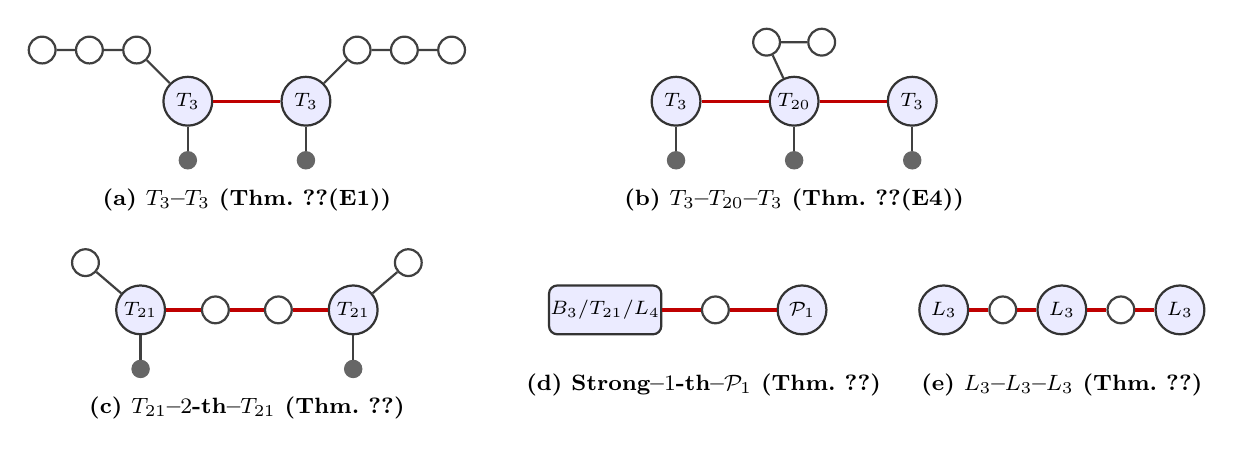
\begin{tikzpicture}[
  core/.style={circle,draw=black!80,fill=blue!8,thick,minimum size=6.2mm,inner sep=0.5pt,font=\scriptsize\bfseries},
  deg2/.style={circle,draw=black!75,fill=white,thick,minimum size=3.4mm,inner sep=0pt},
  leaf/.style={circle,draw=black!60,fill=black!60,minimum size=2.2mm,inner sep=0pt},
  edge/.style={thick,black!75},
  lbl/.style={font=\footnotesize\bfseries,align=center}
]
% (a) T3 -- T3
\begin{scope}[shift={(0,0)}]
  \node[core] (u1) at (0,0) {$T_3$};
  \node[core] (u2) at (1.5,0) {$T_3$};
  \node[deg2] (v1) at (-0.65,0.65) {};
  \node[deg2] (v2) at (-1.25,0.65) {};
  \node[deg2] (v3) at (-1.85,0.65) {};
  \node[deg2] (w1) at (2.15,0.65) {};
  \node[deg2] (w2) at (2.75,0.65) {};
  \node[deg2] (w3) at (3.35,0.65) {};
  \node[leaf] (l1) at (0,-0.75) {};
  \node[leaf] (l2) at (1.5,-0.75) {};
  \draw[edge,red!75!black,very thick] (u1) -- (u2);
  \draw[edge] (u1) -- (v1) -- (v2) -- (v3);
  \draw[edge] (u2) -- (w1) -- (w2) -- (w3);
  \draw[edge] (u1) -- (l1); \draw[edge] (u2) -- (l2);
  \node[lbl] at (0.75,-1.25) {(a) $T_3$--$T_3$ (Thm.~\ref{thm:T3-adj}(E1))};
\end{scope}

% (b) T3 -- T20 -- T3
\begin{scope}[shift={(6.2,0)}]
  \node[core] (t1) at (0,0) {$T_3$};
  \node[core] (t20) at (1.5,0) {$T_{20}$};
  \node[core] (t2) at (3.0,0) {$T_3$};
  \node[deg2] (x1) at (1.15,0.75) {};
  \node[deg2] (x2) at (1.85,0.75) {};
  \node[leaf] (l0) at (1.5,-0.75) {};
  \node[leaf] (l1) at (0,-0.75) {};
  \node[leaf] (l2) at (3.0,-0.75) {};
  \draw[edge,red!75!black,very thick] (t1) -- (t20) -- (t2);
  \draw[edge] (t20) -- (x1) -- (x2);
  \draw[edge] (t1) -- (l1); \draw[edge] (t20) -- (l0); \draw[edge] (t2) -- (l2);
  \node[lbl] at (1.5,-1.25) {(b) $T_3$--$T_{20}$--$T_3$ (Thm.~\ref{thm:T3-adj}(E4))};
\end{scope}

% (c) T21 -- 2-thread -- T21
\begin{scope}[shift={(0,-2.65)}]
  \node[core] (a) at (-0.6,0) {$T_{21}$};
  \node[deg2] (m1) at (0.35,0) {};
  \node[deg2] (m2) at (1.15,0) {};
  \node[core] (b) at (2.1,0) {$T_{21}$};
  \node[deg2] (o1) at (-1.3,0.6) {};
  \node[deg2] (o2) at (2.8,0.6) {};
  \node[leaf] (la) at (-0.6,-0.75) {};
  \node[leaf] (lb) at (2.1,-0.75) {};
  \draw[edge,red!75!black,very thick] (a) -- (m1) -- (m2) -- (b);
  \draw[edge] (a) -- (o1); \draw[edge] (b) -- (o2);
  \draw[edge] (a) -- (la); \draw[edge] (b) -- (lb);
  \node[lbl] at (0.75,-1.25) {(c) $T_{21}$--$2$-th--$T_{21}$ (Thm.~\ref{thm:T21-2th})};
\end{scope}

% (d) Strong -- 1-thread -- P1
\begin{scope}[shift={(5.3,-2.65)}]
  \node[core,minimum width=13mm,rectangle,rounded corners=3pt] (s) at (0,0) {$B_3/T_{21}/L_4$};
  \node[deg2] (mid) at (1.4,0) {};
  \node[core] (p) at (2.5,0) {$\Ppoor$};
  \draw[edge,red!75!black,very thick] (s) -- (mid) -- (p);
  \node[lbl] at (1.25,-0.95) {(d) Strong--$1$-th--$\Ppoor$ (Thm.~\ref{thm:bridge})};
\end{scope}

% (e) L3 -- L3 -- L3
\begin{scope}[shift={(9.6,-2.65)}]
  \node[core] (l1) at (0,0) {$L_3$};
  \node[deg2] (d1) at (0.75,0) {};
  \node[core] (l0) at (1.5,0) {$L_3$};
  \node[deg2] (d2) at (2.25,0) {};
  \node[core] (l2) at (3.0,0) {$L_3$};
  \draw[edge,red!75!black,very thick] (l1) -- (d1) -- (l0) -- (d2) -- (l2);
  \node[lbl] at (1.5,-0.95) {(e) $L_3$--$L_3$--$L_3$ (Thm.~\ref{thm:L3-at-most-one})};
\end{scope}
\end{tikzpicture}
\caption{Key forbidden local configurations in a minimal counterexample under $\mad(G) < 22/9$. Filled small dots indicate $1$-degree leaves; hollow circles indicate $2$-vertices on threads.}
\label{fig:forbidden}
\end{figure}

\subsection{Lemma E: Adjacency Restrictions on \texorpdfstring{$T_3$}{T3} Vertices}

\begin{theorem}[Lemma E: $T_3$ Adjacency Bans]\label{thm:T3-adj}
Let $(G, L)$ be a minimal counterexample.
\begin{enumerate}[label=(E\arabic*),start=0,leftmargin=*,itemsep=2pt]
  \item \emph{(Under $2p \le 5q$.)} No $T_3$ vertex is adjacent to any $3$-vertex.
  \item \emph{(Under $9p \le 22q$.)} No two $T_3$ vertices are adjacent.
  \item \emph{(Under $9p \le 22q$.)} No $T_3$ vertex is adjacent to a $T_{21}$ vertex.
  \item \emph{(Under $9p \le 22q$.)} No $T_3$ vertex is adjacent to a vertex $u_2$ with $d_K(u_2) = 3$ and $n_1(u_2) = 2$.
  \item \emph{(Under $9p \le 22q$.)} No $T_{20}$ vertex is adjacent to two distinct $T_3$ vertices.
\end{enumerate}
\end{theorem}

\begin{proof}
For any $T_3$ vertex $u$, Lemma~\ref{lem:baseline-struct}(ii) gives a unique $3$-thread $u - v_1 - v_2 - v_3 - z$ ($d_G(z) \ge 4$), leaf set $Y = Y(u)$ ($|Y| = d_G(u) - 3 \ge 1$), and two good neighbors.

\medskip
\noindent\textbf{Proof of (E0).} Suppose $u \in T_3$ is adjacent to a $3$-vertex $x_0$, and let $y$ be the other good neighbor of $u$. Delete $S := \{u, v_1, v_2, v_3\} \cup Y$, whose boundary edges are $(u, x_0)$, $(u, y)$, and $(v_3, z)$. Let $F = G[T]$ be the connected component of $G - S$ containing $x_0$. We claim $F \not\cong C_5$: if $F \cong C_5$ with cycle $x_0 c_1 c_2 c_3 c_4 x_0$, then no $c \in T \setminus \{x_0, y\}$ can equal $z$ (else $d_G(c) \le d_F(c) + 1 = 3 < 4 \le d_G(z)$), so $d_G(c) = 2$. Since $y$ can occupy at most one vertex of $\{c_1, c_2, c_3, c_4\}$, either $(c_1, c_2)$ or $(c_4, c_3)$ avoids $y$, yielding a $2^+$-thread at the $3$-vertex $x_0$, contradicting Lemma~\ref{lem:core-struct}(iv). Hence $F$ admits a genuine PCF $L$-coloring $\varphi_F$; since $d_F(x_0) = 2$, its two $F$-neighbors receive distinct colors under $\varphi_F$. Overwriting the $T$-component of an admissible coloring of $G - S$ with $\varphi_F$ yields an admissible coloring $(\varphi, \varphi^*)$ in which $x_0$ already has two distinctly colored neighbors in $G - S$, so $u$ \emph{need not avoid $\varphi^*(x_0)$}. Since $y, z$ are non-isolated in $G - S$, setting $Z_3 := L(v_3) \setminus \{\varphi(z), \varphi^*(z)\}$ ($|Z_3| \ge 2$) and $C_u := L(u) \setminus \{\varphi(y), \varphi^*(y), \varphi(x_0)\}$ ($|C_u| \ge |Y| + 1$) and applying Lemma~\ref{lem:engines}(a) with constant $\delta \equiv \varphi(x_0)$ produces a contradiction.

\medskip
\noindent\textbf{Proof of (E1).} Suppose $u_1, u_2 \in T_3$ are adjacent, with $3$-threads $u_1 - v_1 - v_2 - v_3 - z_1$, $u_2 - w_1 - w_2 - w_3 - z_2$, other good neighbors $y_1, y_2$, and disjoint leaf sets $Y_1, Y_2$.
\begin{itemize}[leftmargin=*,itemsep=2pt]
  \item \emph{Shared $3$-thread ($z_1 = u_2$, so $w_1 = v_3$).} Delete $S := \{u_1, u_2, v_1, v_2, v_3\} \cup Y_1 \cup Y_2$. Only two boundary edges $(u_1, y_1)$ and $(u_2, y_2)$ leave $S$, so no external $3^+$-vertex is isolated. Take $(\varphi, \varphi^*)$ and set $C_i := L(u_i) \setminus \{\varphi(y_i), \varphi^*(y_i)\}$ ($|C_i| \ge |Y_i| + 2$). Pick $\alpha_2 \in C_2$ and $a_r \in L(r) \setminus \{\alpha_2, \varphi(y_2)\}$ for all $r \in Y_2$ (possible by pigeonhole: if every $\alpha \in C_2$ were blocked by some $r \in Y_2$ with $L(r) = \{\alpha, \varphi(y_2)\}$, then $|C_2| \le |Y_2|$, contradiction). Set $Z_3 := L(v_3) \setminus \{\alpha_2, \varphi(y_2)\}$ ($|Z_3| \ge 2$) and $C_1' := C_1 \setminus \{\alpha_2, \varphi(y_2)\}$ ($|C_1'| \ge |Y_1|$). If $|C_1'| \ge |Y_1| + 1$, or if some $r_0 \in Y_1$ satisfies $L(r_0) \cap C_1' = \emptyset$, apply Lemma~\ref{lem:engines}(a) to $u_1$ with $\delta \equiv \alpha_2$, ensuring $\varphi(y_2)$ appears uniquely at $u_2$, contradiction. Otherwise $|C_1'| = |Y_1|$, so $\varphi(y_2) \in C_1$, and no $r \in Y_1$ has $L(r) = \{\varphi(y_2), \varphi(y_1)\}$. Fix $\alpha_1 := \varphi(y_2) \in C_1 \setminus C_2$, choose $a_r \in L(r) \setminus \{\varphi(y_2), \varphi(y_1)\}$ for $r \in Y_1$, set $Z_1 := L(v_1) \setminus \{\varphi(y_2), \varphi(y_1)\}$ ($|Z_1| \ge 2$) and $C_2' := C_2 \setminus \{\varphi(y_1)\}$ ($|C_2'| \ge |Y_2| + 1$), and apply Lemma~\ref{lem:engines}(a) in reverse to $u_2$, making $\varphi(y_1)$ unique at $u_1$, contradiction.
  \item \emph{Disjoint $3$-threads ($z_1 \neq u_2$).} Delete $S := \{u_1, u_2, v_1, v_2, v_3, w_1, w_2, w_3\} \cup Y_1 \cup Y_2$, which has four boundary edges $(u_1, y_1)$, $(u_2, y_2)$, $(v_3, z_1)$, $(w_3, z_2)$. If an isolated external vertex $s \notin S$ exists, then $N_G(s) \subseteq \{u_1, u_2, v_3, w_3\}$ and $d_G(s) \ge 3$ imply $s \in \{z_1, z_2\}$, hence $d_G(s) \ge 4$, forcing $N_G(s) = \{u_1, u_2, v_3, w_3\}$, $d_G(s) = 4$, and $V(G) = \{s\} \cup S$. Then $V(K) = \{s, u_1, u_2, v_1, v_2, v_3, w_1, w_2, w_3\}$ has $|V(K)| = 9$ and $\sum d_K = 4 + 3 + 3 + 6 \cdot 2 = 22$, contradicting Proposition~\ref{prop:core-mad} and $9p \le 22q$. Otherwise take $(\varphi, \varphi^*)$: for each $\alpha_1$, since $|L(u_2) \setminus \{\varphi(y_2), \varphi^*(y_2), \alpha_1\}| \ge |Y_2| + 1$, Lemma~\ref{lem:engines}(a) yields a valid extension on the $u_2$-side with color $\alpha_2 = f_2(\alpha_1)$. Applying the variable-color engine Lemma~\ref{lem:engines}(a) to $u_1$ with $\delta = f_2$ on $C_1 = L(u_1) \setminus \{\varphi(y_1), \varphi^*(y_1)\}$ closes the coloring.
\end{itemize}

\medskip
\noindent\textbf{Proof of (E2).} Suppose $u_1 \in T_3$ is adjacent to $u_2 \in T_{21}$ (having leaf $y_2$, $2$-thread $w_1 - w_2 - z_2$ with $d_G(z_2) \ge 4$, $1$-thread $a_2 - p_2$, and unique good neighbor $u_1$). Delete $S := \{u_1, u_2, v_1, v_2, v_3, w_1, w_2, a_2, y_2\} \cup Y_1$, with four boundary edges $(u_1, y_1)$, $(v_3, z_1)$, $(w_2, z_2)$, $(a_2, p_2)$. Any isolated external vertex $s$ must meet $\{v_3, w_2\}$, forcing $d_G(s) = 4$ and $V(K)$ of size $9$ with $\sum d_K = 4 + 3 + 3 + 6 \cdot 2 = 22$, contradicting $9p \le 22q$. Otherwise take $(\varphi, \varphi^*)$, set $A_a := L(a_2) \setminus \{\varphi(p_2), \varphi^*(p_2)\}$ ($|A_a| \ge 2$) and $c_{\mathrm{f}}(\alpha) \in L(w_2) \setminus \{\varphi(z_2), \varphi^*(z_2), \alpha\}$. For each $\alpha_1$, since $|L(u_2) \setminus \{\alpha_1, \varphi(p_2)\}| \ge 3$, Lemma~\ref{lem:engines}(c) produces a valid $u_2$-side extension with color $\alpha_2 = f_2(\alpha_1)$; applying Lemma~\ref{lem:engines}(a) to $u_1$ with $\delta = f_2$ completes the contradiction.

\medskip
\noindent\textbf{Proof of (E3).} Suppose $u_1 \in T_3$ is adjacent to $u_2$ with $d_K(u_2) = 3$ and $n_1(u_2) = 2$. By~(E0), $d_G(u_2) \ge 4$, so $|Y_2| = d_G(u_2) - 3 \ge 1$. Write the two $1$-threads of $u_2$ as $a_1 - p_1, a_2 - p_2$ and delete $S := \{u_1, u_2, v_1, v_2, v_3, a_1, a_2\} \cup Y_1 \cup Y_2$ (four boundary edges $(u_1, y_1), (v_3, z_1), (a_1, p_1), (a_2, p_2)$). If an external vertex $s$ is isolated, then $s$ meets $\{u_1, v_3\}$, so $d_G(s) \ge 4$ (by~(E0) if $su_1 \in E(G)$, and by Lemma~\ref{lem:core-struct}(iv) if $s = z_1$). Thus $d_G(s) = 4$ and $V(K) = \{s, u_1, u_2, v_1, v_2, v_3, a_1, a_2\}$ has $|V(K)| = 8$ and $\sum d_K = 4 + 3 + 3 + 5 \cdot 2 = 20$, violating $20 \cdot 9 = 180 \ge 176 = 22 \cdot 8$ under $9p \le 22q$. Otherwise take $(\varphi, \varphi^*)$; for each $\alpha_1$, Lemma~\ref{lem:engines}(d) on $C_2(\alpha_1) = L(u_2) \setminus \{\alpha_1, \varphi(p_1), \varphi(p_2)\}$ produces a $u_2$-side extension with color $f_2(\alpha_1)$, and Lemma~\ref{lem:engines}(a) on $u_1$ with $\delta = f_2$ finishes the proof.

\medskip
\noindent\textbf{Proof of (E4).} Suppose $u \in T_{20}$ (with $2$-thread $x_u - y_u - z_u$ and leaf set $Y_u$, $|Y_u| \ge 1$) is adjacent to distinct $u_1, u_2 \in T_3$. By~(E1), $u_1 u_2 \notin E(G)$. Let $u_1 - v_1 - v_2 - v_3 - z_1$ and $u_2 - w_1 - w_2 - w_3 - z_2$ be their $3$-threads, with other good neighbors $y_1, y_2$ and leaf sets $Y_1, Y_2$.
\begin{itemize}[leftmargin=*,itemsep=2pt]
  \item \emph{Shared $3$-thread ($z_1 = u_2$).} Delete $S := \{u, u_1, u_2, x_u, y_u, v_1, v_2, v_3\} \cup Y_u \cup Y_1 \cup Y_2$. Only three boundary edges $(y_u, z_u), (u_1, y_1), (u_2, y_2)$ exit $S$, so no external vertex is isolated (meeting $y_u$ implies $d_G \ge 4 > 3$, while avoiding $y_u$ leaves at most $2$ neighbors). Take $(\varphi, \varphi^*)$, fix $\alpha_2 \in C_2 := L(u_2) \setminus \{\varphi(y_2), \varphi^*(y_2)\}$ with leaves avoiding $\{\alpha_2, \varphi(y_2)\}$, set $Z_3 := L(v_3) \setminus \{\alpha_2, \varphi(y_2)\}$, and for each $\alpha$ use Lemma~\ref{lem:engines}(a) on $u_1$ to get $f_1(\alpha)$. Applying Lemma~\ref{lem:engines}(b) to $u$ on $C_u := L(u) \setminus \{\alpha_2, \varphi(y_2)\}$ ($|C_u| \ge |Y_u| + 2$) with $\delta_1 = f_1, \delta_2 \equiv \alpha_2$ ensures $\varphi(y_2)$ is unique at $u_2$ and closes the coloring.
  \item \emph{Disjoint $3$-threads ($z_1 \neq u_2$).} Delete $S := \{u, u_1, u_2, x_u, y_u, v_1, v_2, v_3, w_1, w_2, w_3\} \cup Y_u \cup Y_1 \cup Y_2$ (five boundary edges $(y_u, z_u), (u_1, y_1), (v_3, z_1), (u_2, y_2), (w_3, z_2)$). Every isolated external vertex must meet $\{y_u, v_3, w_3\}$ and hence has degree at least $4$; since $4 + 4 > 5$, at most one isolated external vertex $s_0$ can exist.
  \begin{enumerate}[label=\arabic*.,leftmargin=*,itemsep=1pt]
    \item \emph{No isolated vertex:} For each $\alpha$, Lemma~\ref{lem:engines}(a) yields $f_1(\alpha), f_2(\alpha)$ for $u_1, u_2$, and Lemma~\ref{lem:engines}(b) on $C_u = L(u)$ closes $u$.
    \item \emph{Unique isolated vertex $s_0 = z_u$:} Fix $c_{y_u} \in L(y_u) \setminus \{\varphi(z_u)\}$ and treat $c_{y_u}$ as the avoided color at $s_0$ for all other boundary neighbors (so $y_u$ becomes the unique neighbor of $s_0$ with color $c_{y_u}$). Applying Lemma~\ref{lem:engines}(a) for $u_1, u_2$ and Lemma~\ref{lem:engines}(b) on $C_u = L(u) \setminus \{c_{y_u}\}$ ($|C_u| \ge |Y_u| + 3$) with $c_{\mathrm{f}} \equiv c_{y_u}$ closes the coloring.
    \item \emph{Unique isolated vertex $s_0 \neq z_u$:} Then $s_0 y_u \notin E(G)$, so $d_G(s_0) \ge 4$ forces $N_G(s_0) = \{u_1, v_3, u_2, w_3\}$ and $s_0 = y_1 = z_1 = y_2 = z_2$. Set $Z_1 := L(v_3) \setminus \{\varphi(s_0)\}$ ($|Z_1| \ge 3$). For each $\alpha$, apply the \emph{avoid variant} of Lemma~\ref{lem:engines}(a) to $u_1$ on $L(u_1) \setminus \{\varphi(s_0), \alpha\}$ (size $\ge |Y_1| + 2$) to pick $\alpha_1 = f_1(\alpha)$ and $c_3 \in Z_1 \setminus \{\alpha_1\}$; then apply Lemma~\ref{lem:engines}(a) to $u_2$ with $Z_2(\alpha) = L(w_3) \setminus \{\varphi(s_0), f_1(\alpha)\}$ and $C_2(\alpha) = L(u_2) \setminus \{\varphi(s_0), f_1(\alpha), \alpha\}$ so that $f_2(\alpha) \neq f_1(\alpha)$ and $d_3 \neq f_1(\alpha)$ (making $f_1(\alpha)$ unique at $s_0$!). Finally, Lemma~\ref{lem:engines}(b) on $C_u = L(u)$ closes $u$. \qedhere
  \end{enumerate}
\end{itemize}
\end{proof}

\subsection{Lemma D2: No \texorpdfstring{$2$}{2}-Thread Between Two \texorpdfstring{$T_{21}$}{T21} Vertices}

The remaining three theorems in this section all hold under the weaker assumption $2p \le 5q$ ($\mad(G) < 5/2$).

\begin{theorem}[Lemma D2: No $2$-Thread Between $T_{21}$ Vertices]\label{thm:T21-2th}
Under $2p \le 5q$, no two $T_{21}$ vertices $u, v$ are joined by a $2$-thread $u - t_1 - t_2 - v$.
\end{theorem}

\begin{proof}
Write the remaining neighbors of $u$ as leaf $y_1$, $1$-thread $a_1 - p_1$, and good neighbor $x_1$; similarly for $v$ write $y_2$, $a_2 - p_2$, and $x_2$. Delete $S := \{u, v, t_1, t_2, y_1, y_2, a_1, a_2\}$. Notice the elementary fact ($\star$): given three fixed colors $c_1, c_2, c_3$ and any two distinct choices $c_4 \neq c_4'$, at least one of $[c_1, c_2, c_3, c_4]$ or $[c_1, c_2, c_3, c_4']$ has a unique color.

If $uv \in E(G)$ or $a_1 = a_2$, then at most two boundary edges leave $S$, so no external $3^+$-vertex is isolated. Choosing $\alpha \in L(u)$ avoiding $L(y_1)$ and external color constraints (possible since $|L(u)| = 5$), choosing $\beta \in L(v)$ similarly, coloring $a_1, a_2, t_1, t_2$ greedily, and finishing $y_1, y_2$ via~($\star$) yields a PCF $L$-coloring in all three coinciding cases.

Assume now that $uv \notin E(G)$ and $a_1 \neq a_2$, so four boundary edges $(u, x_1)$, $(v, x_2)$, $(a_1, p_1)$, and $(a_2, p_2)$ leave $S$. Let $(\varphi, \varphi^*)$ be an admissible coloring of $G - S$.
\begin{itemize}[leftmargin=*,itemsep=2pt]
  \item \emph{An isolated external vertex $w \notin S$ exists.} Since $d_G(w) \ge 3$ and $3 + 3 > 4$, $w$ is unique, and by pigeonhole (without loss of generality) $\{u, a_1\} \subseteq N_G(w)$, i.e., $x_1 = p_1 = w$ (lifting $\varphi^*(w)$ at $u, a_1$). Greedily choose valid colors $\alpha$ on $v$, $c_{a_2}$ on $a_2$, and $c_{y_2}$ on $y_2$. Set $G_u := L(u) \setminus (\{\varphi(w)\} \cup L(y_1))$ ($|G_u| \ge 2$). If $d_G(w) = 4$ (so $N_G(w) = \{u, a_1, v, a_2\}$): either pick $\gamma \in G_u \setminus \{\alpha, c_{a_2}\}$ and $c_{a_1} \in L(a_1) \setminus \{\varphi(w), \gamma\}$ (making $\gamma$ unique at $w$), or else $G_u = \{\alpha, c_{a_2}\}$ and picking $\gamma = \alpha$ with $c_{a_1} \in L(a_1) \setminus \{\varphi(w), \alpha, c_{a_2}\}$ makes $c_{a_1}$ unique at $w$. If $d_G(w) = 3$, any $\gamma \in G_u$ and $c_{a_1} \in L(a_1) \setminus \{\varphi(w), \gamma\}$ give $\gamma \neq c_{a_1}$ (PCF at $w$). Finish $t_2$ via~($\star$) for $v$, pick $c_{t_1} \in L(t_1) \setminus \{\gamma, \alpha, c_{t_2}\}$, and finish $y_1$ via~($\star$) for $u$.
  \item \emph{No isolated external vertex exists.} Set $C_1 := L(u) \setminus \{\varphi(x_1), \varphi^*(x_1), \varphi(p_1)\}$ ($|C_1| \ge 2$, $\beta_1 := \varphi(x_1) \notin C_1$), $C_2 := L(v) \setminus \{\varphi(x_2), \varphi^*(x_2), \varphi(p_2)\}$ ($|C_2| \ge 2$), and $A_i := L(a_i) \setminus \{\varphi(p_i), \varphi^*(p_i)\}$ ($|A_i| \ge 2$). For any $(\gamma, \alpha) \in C_1 \times C_2$, we can always pick $c_{y_2} \in L(y_2) \setminus \{\alpha\}$, $c_{a_2} \in A_2 \setminus \{\alpha\}$, and $c_{t_2} \in L(t_2) \setminus \{\alpha, \gamma\}$ satisfying PCF at $v$ via~($\star$). If some $\gamma \in C_1$ has $|L(y_1) \setminus \{\gamma\}| \ge 2$ or $|A_1 \setminus \{\gamma\}| \ge 2$, pick any $\alpha \in C_2$, complete $v$'s side, choose $c_{t_1} \in L(t_1) \setminus \{\gamma, \alpha, c_{t_2}\}$, and use the $2$-choice set on $y_1$ or $a_1$ via~($\star$) to satisfy PCF at $u$. Otherwise, picking distinct $\gamma_1 \neq \gamma_2 \in C_1$ and $\alpha_1 \neq \alpha_2 \in C_2$ forces $L(y_1) = A_1 = \{\gamma_1, \gamma_2\}$. Some pair $(\gamma, \alpha) \in \{\gamma_1, \gamma_2\} \times \{\alpha_1, \alpha_2\}$ must satisfy $|L(t_1) \setminus \{\gamma, \alpha, \beta_1\}| \ge 2$ (otherwise all four triples $\{\gamma, \alpha, \beta_1\}$ are $3$-element subsets of $L(t_1)$, forcing $\{\gamma_1, \gamma_2, \alpha_1, \alpha_2, \beta_1\} \subseteq L(t_1)$ of size $5 > 4$, impossible!). Taking this pair (say $\gamma = \gamma_1$), we get $c_{y_1} = c_{a_1} = \gamma_2 \neq \beta_1$; completing $v$'s side and picking $c_{t_1} \in (L(t_1) \setminus \{\gamma, \alpha, \beta_1\}) \setminus \{c_{t_2}\}$ leaves $\beta_1$ unique at $u$. \qedhere
\end{itemize}
\end{proof}

\subsection{Pre-Exclusions, Strong-Side Abstraction, and Lemmas D1 and C}

Recall $\Ppoor := \{L_3, B_3, T_{21}, L_4\}$. Note that if two vertices in $\Ppoor$ are adjacent, then both must be $T_{21}$ (since $L_3, B_3, L_4$ have no good neighbors and no vertex in $\Ppoor$ is bad). We first rule out six small overlapping configurations so that the local neighborhoods on opposite ends of a $1$-thread bridge are guaranteed to be disjoint.

\begin{lemma}[Six Pre-Exclusion Configurations]\label{lem:pre-excl}
Under $2p \le 5q$, none of the following occurs in $G$:
\begin{enumerate}[label=(\roman*),leftmargin=*,itemsep=1pt]
  \item Two distinct vertices $u, v \in \{L_3, L_4\}$ sharing all three $1$-threads.
  \item Two distinct $B_3$ vertices sharing their bad neighbor and both $1$-threads.
  \item Two distinct vertices $u, v \in \Ppoor$ joined by two distinct $1$-threads $a_1, a_2$.
  \item Two adjacent $T_{21}$ vertices joined additionally by a $1$-thread.
  \item Two $B_3$ vertices sharing their bad neighbor and joined by a $1$-thread.
  \item Three pairwise distinct $L_3$ vertices pairwise joined by $1$-threads (a subdivided $L_3$-triangle).
\end{enumerate}
\end{lemma}

\begin{proof}
(i)--(ii) The natural vertex sets $S$ are closed ($S = V(G)$): pick $\alpha \in L(u)$ (avoiding $L(y_u)$ if $L_4$), $\beta \in L(v) \setminus \{\alpha\}$ (avoiding $L(y_v)$ if $L_4$), color the shared bad vertex via Lemma~\ref{lem:bad-ext}(b) in~(ii), assign distinct colors $c_1 \neq c_2$ on $a_1, a_2$ (giving PCF at $u, v$ for $L_3, B_3$), and finish any leaves via~($\star$).

(iii) Neither $u$ nor $v$ can be $T_{21}$ (which has $n_1 = 1$). By~(i)--(ii), $u$ and $v$ do not share their third core neighbor. Each remaining side $S_{\mathrm{rem}}(x)$ ($x \in \{u, v\}$) has only one boundary edge $(e_x, p_x)$ with $p_x$ outside the opposite side, and admits a safe color set $A_x \subseteq L(x)$ of size $\ge 2$ (size $\ge 3$ for $L_3$, $4$ for $B_3$ via Lemma~\ref{lem:bad-ext}(b), and $\ge 2$ for $L_4$ avoiding $L(y_x)$ and $\varphi(p_x)$). Deleting $S = \{a_1, a_2\} \cup S_{\mathrm{rem}}(u) \cup S_{\mathrm{rem}}(v)$ leaves only two boundary edges, so no external vertex is isolated; picking $\alpha \in A_u$, $\beta \in A_v \setminus \{\alpha\}$, and distinct colors on $a_1, a_2$ closes both sides.

(iv) By Theorem~\ref{thm:T21-2th}, the $2$-threads of $u$ and $v$ are disjoint. Deleting $S := \{u, v, a, y_1, y_2\} \cup \{t_1, t_2, s_1, s_2\}$ leaves only two boundary edges, so coloring greedily while avoiding $L(y_1)$ and $L(y_2)$, and finishing $y_1, y_2$ via~($\star$), closes $G$.

(v) By~(iii), the remaining $1$-threads $a_1 - p_1, a_2 - p_2$ are disjoint with $p_1, p_2 \notin \{u, v, b\}$. Deleting $S = \{u, v, a, a_1, a_2, b\} \cup Y(b)$ leaves two boundary edges; pick $\alpha \in L(u) \setminus \{\varphi(p_1)\}$, $\beta \in L(v) \setminus \{\varphi(p_2), \alpha\}$, color $b$ and $Y(b)$ via Lemma~\ref{lem:bad-ext}(b) with color $c_b$, color $a_1, a_2$ greedily, and pick $c_a \in L(a) \setminus \{\alpha, \beta, c_b\}$ (ensuring PCF at $u, v$).

(vi) By~(iii), the three outward $1$-threads $a_3 - p_0$, $b_1 - p_1$, and $b_2 - p_2$ exit the $9$-vertex set $S := \{u, v_1, v_2, a_1, a_2, a', a_3, b_1, b_2\}$ via three boundary edges. Pick $\gamma \in L(u) \setminus \{\varphi(p_0)\}$, $\alpha_1 \in L(v_1) \setminus \{\varphi(p_1), \gamma\}$, and $\alpha_2 \in L(v_2) \setminus \{\varphi(p_2), \gamma, \alpha_1\}$. If an external vertex $w$ is isolated, then $d_G(w) = 3$ and $N_G(w) = \{a_3, b_1, b_2\}$, so pick $c_3 \in L(a_3) \setminus \{\gamma, \varphi(w)\}$, $d_1 \in L(b_1) \setminus \{\alpha_1, \varphi(w), c_3\}$ (giving PCF at $w$), and $d_2 \in L(b_2) \setminus \{\alpha_2, \varphi(w)\}$; otherwise color $a_3, b_1, b_2$ greedily avoiding $\varphi, \varphi^*$. Finally choose $c_1 \in L(a_1) \setminus \{\gamma, \alpha_1, c_3\}$, $c' \in L(a') \setminus \{\alpha_1, \alpha_2, d_1\}$, and $c_2 \in L(a_2) \setminus \{\gamma, \alpha_2, d_2\}$ to satisfy PCF at $u, v_1, v_2$.
\end{proof}

Next we record two pure combinatorial singleton bounds for one side of a $1$-thread $u - a - v$ (with $|L(a)| = 4$).

\begin{lemma}[Side Reachability Singleton Bounds]\label{lem:side-bounds}
Let $|L_a| = 4$ and let $C$ be any finite color set.
\begin{enumerate}[label=(\alph*),leftmargin=*,itemsep=2pt]
  \item \emph{($L_3/B_3$ side.)} If $|C_2|, |A_2|, |A_3| \ge 2$ and
  \[\begin{aligned}
    G_{\mathrm{pair}}(\gamma) := \bigl\{c_a \in L_a \setminus \{\gamma\} :\ & \exists \alpha \in C_2 \setminus \{\gamma, c_a\},\ \exists c_2 \in A_2 \setminus \{\alpha\},\\
    & \exists c_3 \in A_3 \setminus \{\alpha\},\ \neg(c_a = c_2 = c_3)\bigr\},
  \end{aligned}\]
  then $G_{\mathrm{pair}}(\gamma) \neq \emptyset$ for all $\gamma$, and $|\{\gamma \in C : |G_{\mathrm{pair}}(\gamma)| = 1\}| \le 2$.
  \item \emph{($L_4/T_{21}$ side.)} If $|C_v| \ge 3$, $|L_y| = 2$, and for every $\alpha \in C_v$ there exists a valid pair $(c_1, c_2)$ satisfying a side predicate $P(\alpha, c_1, c_2)$, then
  \[\begin{aligned}
    G_{\mathrm{leaf}}(\gamma) := \bigl\{c_a \in L_a \setminus \{\gamma\} :\ & \exists \alpha \in C_v \setminus \{\gamma, c_a\},\ \exists c_y \in L_y \setminus \{\alpha\},\\
    & \exists c_1, c_2,\ P(\alpha, c_1, c_2) \land \mathrm{HasUnique}([c_1, c_2, c_y, c_a])\bigr\}
  \end{aligned}\]
  is nonempty for all $\gamma$, and $|\{\gamma \in C : |G_{\mathrm{leaf}}(\gamma)| = 1\}| \le 1$.
\end{enumerate}
\end{lemma}

\begin{proof}
(a) If $|G_{\mathrm{pair}}(\gamma)| = 1$, then for any $\alpha \in C_2 \setminus \{\gamma\}$ we must have $A_2 \setminus \{\alpha\} = A_3 \setminus \{\alpha\} = \{c_0\}$ (else two distinct colors $c_2 \neq c_3$ make every $c_a \in L_a \setminus \{\gamma, \alpha\}$ valid, giving $|G_{\mathrm{pair}}(\gamma)| \ge 2$). Hence $|A_2| = 2$ and $A_2 = \{\alpha, c_0\}$, so every $c_a \in L_a \setminus (\{\gamma\} \cup A_2)$ lies in $G_{\mathrm{pair}}(\gamma)$; since $|G_{\mathrm{pair}}(\gamma)| = 1$ and $|L_a| = 4$, we must have $\{\gamma\} \cup A_2 \subseteq L_a$ with $\gamma \notin A_2$, placing $\gamma$ inside the $2$-element set $L_a \setminus A_2$.

(b) If $|G_{\mathrm{leaf}}(\gamma)| = 1$, then every $\alpha \in C_v \setminus \{\gamma\}$ must lie in $L_y$ (else $|L_y \setminus \{\alpha\}| = 2$, and by~($\star$) every $c_a \in L_a \setminus \{\gamma, \alpha\}$ lies in $G_{\mathrm{leaf}}(\gamma)$, size $\ge 2$). Thus $C_v \setminus \{\gamma\} \subseteq L_y$. If two distinct $\gamma_1 \neq \gamma_2$ gave singletons, then $C_v = (C_v \setminus \{\gamma_1\}) \cup (C_v \setminus \{\gamma_2\}) \subseteq L_y$, contradicting $|C_v| \ge 3 > 2 = |L_y|$.
\end{proof}

\begin{theorem}[Lemma D1: Unified $1$-Thread Bridging Bans]\label{thm:bridge}
Under $2p \le 5q$, no vertex $u \in \{B_3, T_{21}, L_4\}$ is joined by a $1$-thread $u - a - v$ to any vertex $v \in \Ppoor = \{L_3, B_3, T_{21}, L_4\}$.
\end{theorem}

\begin{proof}
For every endpoint $x \in \Ppoor$ incident to a $1$-thread $a$, define its local side block $S_{\mathrm{side}}(x)$ with exactly two boundary edges $(e_1, p_1), (e_2, p_2)$:
\begin{itemize}[leftmargin=*,itemsep=1pt]
  \item $L_3$: $S_{\mathrm{side}} = \{x, b_1, b_2\}$, exits $(b_1, p_1), (b_2, p_2)$;
  \item $B_3$: $S_{\mathrm{side}} = \{x, a', b\} \cup Y(b)$, exits $(a', p_1), (b, h)$;
  \item $L_4$: $S_{\mathrm{side}} = \{x, y, b_1, b_2\}$, exits $(b_1, p_1), (b_2, p_2)$;
  \item $T_{21}$: $S_{\mathrm{side}} = \{x, y, t_1, t_2\}$, exits $(x, x'), (t_2, z)$ ($d_G(z) \ge 4$).
\end{itemize}
By Lemma~\ref{lem:pre-excl}(iii)--(v), Theorem~\ref{thm:T21-2th}, and Lemma~\ref{lem:baseline-struct}(i), the two blocks $S_{\mathrm{side}}(u)$ and $S_{\mathrm{side}}(v)$ are disjoint, and neither side's external endpoints $p_1, p_2$ lie in the opposite side. Set $S := \{a\} \cup S_{\mathrm{side}}(u) \cup S_{\mathrm{side}}(v)$, which has four boundary edges. Let $(\varphi, \varphi^*)$ be an admissible coloring of $G - S$.

All four classes in $\Ppoor$ satisfy three uniform side properties:
\begin{enumerate}[label=(S\arabic*),leftmargin=*,itemsep=1pt]
  \item \emph{Reachability (\code{hgoodA}):} There is a nonempty family $G_a(\gamma) \subseteq L(a) \setminus \{\gamma\}$ with $|\{\gamma \in C : |G_a(\gamma)| = 1\}| \le 2$ (via Lemma~\ref{lem:side-bounds}(a) for $L_3, B_3$, using Lemma~\ref{lem:bad-ext}(a) on $b$, and Lemma~\ref{lem:side-bounds}(b) for $L_4, T_{21}$) such that any $c_a \in G_a(\gamma)$ extends to $S_{\mathrm{side}}$ avoiding $\gamma$ on $x$.
  \item \emph{Greedy dual-exit (\code{hgreedy}):} $S_{\mathrm{side}}$ admits a valid coloring $\psi_s$ together with \emph{two distinct} colors $c_{a,1} \neq c_{a,2} \in L(a) \setminus \{\psi_s(x)\}$ either of which preserves PCF on all of $S_{\mathrm{side}}$.
  \item \emph{Isolated double-exit (\code{hisoDouble}):} When both exits of a side land on a single isolated external vertex $w$ ($p_1 = p_2 = w$, lifting $\varphi^*(w)$), given any opposite color $\gamma_{\mathrm{opp}}$, any two distinct choices $c_{a,1} \neq c_{a,2} \in L(a) \setminus \{\gamma_{\mathrm{opp}}\}$, and the list $B_w$ of colors already assigned to $w$'s other $1$ or $2$ neighbors in $S$, there exist $c_a \in \{c_{a,1}, c_{a,2}\}$ and a valid coloring of $S_{\mathrm{side}}$ ensuring $\mathrm{HasUnique}(B_w \cup [\psi(e_1), \psi(e_2)])$ (via elementary $2$-set pairing \code{pair_double_pcf} for $L_3, L_4$, Lemma~\ref{lem:bad-ext}(b) for $B_3$, and~($\star$) for $T_{21}$).
\end{enumerate}

\emph{Case 1: an isolated external vertex $w \notin S$ exists.} Since $d_G(w) \ge 3$ and $3 + 3 > 4$, $w$ is unique, and by pigeonhole $w$ receives both exits from at least one side (say $v$'s side, symmetrically if $u$'s). Color $u$'s side by~(S2) to get $(\gamma, c_{a,1}, c_{a,2})$ and the list $B_w$ of length $1$ or $2$; then close $v$'s side, $a$, and $w$ simultaneously via~(S3).

\emph{Case 2: no isolated external vertex exists.} Here the asymmetry between $\{B_3, T_{21}, L_4\}$ and $L_3$ is decisive: every $u \in \{B_3, T_{21}, L_4\}$ satisfies the \emph{strong-side property} (\code{IsStrong}): there is a set $C_u \subseteq L(u)$ of size $|C_u| \ge 3$ (namely $L(u) \setminus \{\varphi(p_1)\}$ for $B_3$, $L(u) \setminus \{\varphi(p_1), \varphi(p_2)\}$ for $L_4$, and $L(u) \setminus \{\varphi(x'), \varphi^*(x')\}$ for $T_{21}$; whereas $L_3$ has only $|L(u) \setminus \{\varphi(p_1), \varphi(p_2)\}| \ge 2$) such that for every $\gamma \in C_u$ and every subset $G_a \subseteq L(a) \setminus \{\gamma\}$ of size $\ge 2$, some $c_a \in G_a$ extends to a valid PCF coloring of $S_{\mathrm{side}}(u)$ with $\psi(u) = \gamma$. (For $B_3$ this uses Lemma~\ref{lem:bad-ext}(b) on $b$; for $L_4$ and $T_{21}$ this uses $|G_a| \ge 2$ together with~($\star$) after fixing the non-$a$ neighbors of $u$.)

Now apply~(S1) to $v$'s side to obtain $G_a(\cdot)$. Since $|C_u| \ge 3$ and at most $2$ colors $\gamma \in C_u$ satisfy $|G_a(\gamma)| = 1$, there exists $\gamma \in C_u$ with $|G_a(\gamma)| \ge 2$. By the strong-side property of $u$, choose $c_a \in G_a(\gamma)$ and a valid coloring of $S_{\mathrm{side}}(u)$ with $\psi(u) = \gamma$; then~(S1) extends $(\gamma, c_a)$ to $S_{\mathrm{side}}(v)$, contradicting minimality.
\end{proof}

\begin{theorem}[Lemma C: At Most One $L_3$ Partner]\label{thm:L3-at-most-one}
Under $2p \le 5q$, every $L_3$ vertex $u$ is joined by $1$-threads to at most one $L_3$ vertex.
\end{theorem}

\begin{proof}
Suppose $u \in L_3$ is joined via distinct $1$-threads $a_1, a_2$ to $L_3$ vertices $v_1, v_2$. By Lemma~\ref{lem:pre-excl}(iii), $v_1 \neq v_2$. Write $u$'s third $1$-thread as $a_3 - p_0$, $v_1$'s other two as $b_1 - q_1, b_2 - q_2$, and $v_2$'s other two as $d_1 - r_1, d_2 - r_2$. By Lemma~\ref{lem:pre-excl}(iii),(vi), all five external endpoints lie outside $\{u, v_1, v_2\}$, so $S := \{u, v_1, v_2, a_1, a_2, a_3, b_1, b_2, d_1, d_2\}$ consists of $10$ distinct vertices with five boundary edges $(a_3, p_0), (b_1, q_1), (b_2, q_2), (d_1, r_1), (d_2, r_2)$. Let $(\varphi, \varphi^*)$ be an admissible coloring of $G - S$.

\emph{Case 1: no isolated external vertex exists.} Apply Lemma~\ref{lem:side-bounds}(a) to the $v_1$-branch and $v_2$-branch to obtain nonempty families $G_1(\gamma) \subseteq L(a_1) \setminus \{\gamma\}$ and $G_2(\gamma) \subseteq L(a_2) \setminus \{\gamma\}$, each having at most $2$ singletons. Since $|C_u| := |L(u) \setminus \{\varphi(p_0)\}| \ge 3$, pick $\gamma \in C_u$ with $|G_1(\gamma)| \ge 2$. Choose any $c_2 \in G_2(\gamma)$, then $c_1 \in G_1(\gamma) \setminus \{c_2\}$ (so $c_1 \neq c_2$, ensuring PCF at $u$), and $c_3 \in L(a_3) \setminus \{\varphi(p_0), \varphi^*(p_0), \gamma\}$; expanding $G_1, G_2$ completes a PCF $L$-coloring of $G$.

\emph{Case 2: an isolated external vertex $w \notin S$ exists.} Since $d_G(w) \ge 3$ and $3 + 3 > 5$, $w$ is unique.
\begin{itemize}[leftmargin=*,itemsep=2pt]
  \item If $|N_G(w) \cap \{b_1, b_2\}| \le 1$ and $|N_G(w) \cap \{d_1, d_2\}| \le 1$, then $d_G(w) \ge 3$ forces $d_G(w) = 3$ with $N_G(w) = \{a_3, b_i, d_j\}$ for some $i, j$. Thus $w$ itself is an $L_3$ vertex, and $\{u, v_1, w\}$ forms a subdivided $L_3$-triangle via $(a_1, a_3, b_i)$, contradicting Lemma~\ref{lem:pre-excl}(vi).
  \item Otherwise, without loss of generality $\{b_1, b_2\} \subseteq N_G(w)$, so $q_1 = q_2 = w$ (lifting $\varphi^*(w)$). Choose $\alpha_2 \in L(v_2) \setminus \{\varphi(r_1), \varphi(r_2)\}$, $\gamma \in L(u) \setminus \{\varphi(p_0), \alpha_2\}$, and $\alpha_1 \in L(v_1) \setminus \{\gamma, \varphi(w)\}$. If $d_G(w) = 5$ (so $p_0 = r_1 = r_2 = w$), pick $c_{d_1} \in L(d_1) \setminus \{\varphi(w), \alpha_2\}$, force the other four neighbors $d_2, a_3, b_1, b_2$ of $w$ to avoid $c_{d_1}$ (making $c_{d_1}$ unique at $w$ and ensuring $c_{d_2} \neq c_{d_1}$ for $v_2$), and pick $c_2 \in L(a_2) \setminus \{\gamma, \alpha_2, c_3\}$ and $c_1 \in L(a_1) \setminus \{\gamma, \alpha_1, c_{b_1}\}$. If $d_G(w) \in \{3, 4\}$, greedily color $a_3, d_1, d_2$, pick $c_2 \in L(a_2) \setminus \{\gamma, \alpha_2, c_{d_1}\}$ (PCF at $v_2$) and $c_1 \in L(a_1) \setminus \{\gamma, \alpha_1, c_2\}$ (PCF at $u$), and finally color $(b_1, b_2)$ from $L(b_i) \setminus \{\alpha_1, \varphi(w)\}$ (each of size $\ge 2$) so that both $v_1$ and $w$ satisfy PCF (using the same elementary $2$-set pairing \code{pair_double_pcf}). \qedhere
\end{itemize}
\end{proof}

%==============================================================================
\section{Proof of Theorem~\ref{thm:main} via \texorpdfstring{$36$}{36}-Scaled Discharging}\label{sec:discharging}
%==============================================================================

Suppose for contradiction that Theorem~\ref{thm:main} is false, and let $(G, L)$ be a minimal counterexample with $p = 22, q = 9$ (note $2 \cdot 22 \le 5 \cdot 9$ and $9 \cdot 22 \le 22 \cdot 9$, so all results of Sections~\ref{sec:universal}--\ref{sec:lemmas-CDE} apply). By Lemma~\ref{lem:core-struct}(i), $V(K) = \{v \in V(G) : d_G(v) \ge 2\}$ is nonempty. Assign to every core vertex $u \in V(K)$ the integer initial charge (scaling $d_K(u) - 22/9$ by $36$):
\[
  \ch(u) := 36\, d_K(u) - 88.
\]
By Proposition~\ref{prop:core-mad} with $(p, q) = (22, 9)$, we have $9 \sum_{u \in V(K)} d_K(u) < 22|V(K)|$, and hence
\begin{equation}\label{eq:neg-sum}
  \sum_{u \in V(K)} \ch(u) = 4\Bigl(9 \sum_{u \in V(K)} d_K(u) - 22|V(K)|\Bigr) < 0.
\end{equation}

We redistribute charge among vertices of $V(K)$ according to three integer rules (Figure~\ref{fig:discharging}):
\begin{itemize}[leftmargin=*,itemsep=3pt]
  \item \textbf{Rule R1 (Anchors $\to$ $2$-vertices on threads).} By Lemma~\ref{lem:core-struct}(iii), every $2$-vertex $x \in V(K)$ belongs to a unique $k$-thread ($k \in \{1, 2, 3\}$) with two distinct $3^+$-anchors $u, w$. Each anchor sends charge to $x$ as follows:
  \begin{enumerate}[label=\textbf{R1\alph*.},leftmargin=*,itemsep=1pt]
    \item \emph{$1$-thread:} If one anchor lies in $\Ppoor = \{L_3, B_3, T_{21}, L_4\}$ and the other does not, the $\Ppoor$-anchor sends $6$ and the non-$\Ppoor$-anchor sends $10$; otherwise both anchors send $8$.
    \item \emph{$2$-thread:} If one anchor is $T_{21}$ and the other is not, the $T_{21}$-anchor sends $7$ to each of the two internal $2$-vertices ($14$ total) and the other sends $9$ to each ($18$ total); otherwise both send $8$ to each ($16$ total).
    \item \emph{$3$-thread:} Each anchor sends $8$ to each of the three internal $2$-vertices ($24$ total).
  \end{enumerate}
  \item \textbf{Rule R2 (Good $\to$ Bad).} Every good core vertex sends $8$ to each adjacent bad core vertex.
  \item \textbf{Rule R3 (Good $\to$ $T_3$).} Every good core vertex sends $2$ to each adjacent $T_3$ vertex.
\end{itemize}

\begin{figure}[t]
\centering
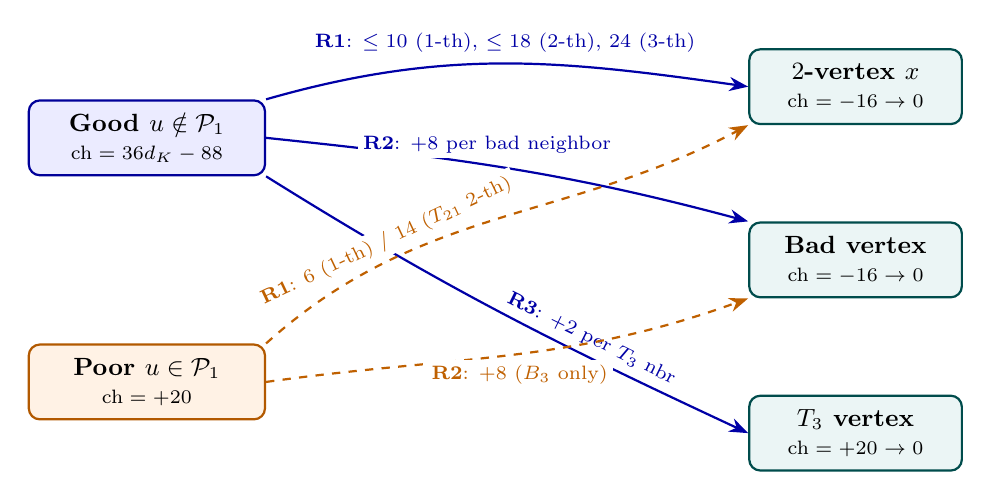
\begin{tikzpicture}[
  box/.style={rectangle,rounded corners=4pt,draw=black!80,fill=white,thick,minimum height=9.5mm,font=\small\bfseries,align=center},
  good/.style={box,fill=blue!8,draw=blue!60!black,minimum width=30mm},
  poor/.style={box,fill=orange!10,draw=orange!70!black,minimum width=30mm},
  sink/.style={box,fill=teal!8,draw=teal!60!black,minimum width=27mm},
  arr/.style={-{Stealth[length=2.4mm]},thick,black!75},
  albl/.style={font=\scriptsize,fill=white,inner sep=1.8pt}
]
\node[good] (G) at (0, 1.55) {Good $u \notin \Ppoor$\\[-1pt]\scriptsize $\ch = 36 d_K - 88$};
\node[poor] (P) at (0,-1.55) {Poor $u \in \Ppoor$\\[-1pt]\scriptsize $\ch = +20$};

\node[sink] (D2) at (9.0, 2.2) {$2$-vertex $x$\\[-1pt]\scriptsize $\ch = -16 \to 0$};
\node[sink] (B)  at (9.0, 0.0) {Bad vertex\\[-1pt]\scriptsize $\ch = -16 \to 0$};
\node[sink] (T3) at (9.0,-2.2) {$T_3$ vertex\\[-1pt]\scriptsize $\ch = +20 \to 0$};

\draw[arr,blue!65!black] (G.north east) to[out=16,in=172] node[albl,pos=0.5,above=2pt] {\textbf{R1}: $\le 10$ ($1$-th), $\le 18$ ($2$-th), $24$ ($3$-th)} (D2.west);
\draw[arr,blue!65!black] (G.east) to[out=-6,in=165] node[albl,pos=0.45,above=2pt] {\textbf{R2}: $+8$ per bad neighbor} (B.north west);
\draw[arr,blue!65!black] (G.south east) to[out=-32,in=155] node[albl,pos=0.68,sloped,above=1pt] {\textbf{R3}: $+2$ per $T_3$ nbr} (T3.west);

\draw[arr,orange!75!black,dashed] (P.north east) to[out=42,in=208] node[albl,pos=0.28,sloped,above=1pt] {\textbf{R1}: $6$ ($1$-th) / $14$ ($T_{21}$ $2$-th)} (D2.south west);
\draw[arr,orange!75!black,dashed] (P.east) to[out=8,in=200] node[albl,pos=0.52,below=2pt] {\textbf{R2}: $+8$ ($B_3$ only)} (B.south west);
\end{tikzpicture}
\caption{Charge flow of the $36$-scaled integer discharging rules \textbf{R1}--\textbf{R3} on the core subgraph $K$.}
\label{fig:discharging}
\end{figure}

Let $\ch'(u)$ denote the final charge of $u \in V(K)$. Since charge is conserved ($\sum_{u \in V(K)} \ch'(u) = \sum_{u \in V(K)} \ch(u)$), proving $\ch'(u) \ge 0$ for every $u \in V(K)$ contradicts~\eqref{eq:neg-sum}. Notice first that every $3^+$-vertex $u$ sends at most $10 n_1(u) + 18 n_2(u) + 24 n_3(u)$ by \textbf{R1}, and every good vertex $u$ sends at most $8 b(u) + 2 t_{T_3}(u)$ by \textbf{R2}--\textbf{R3}, where $t_{T_3}(u) \le g(u)$ is the number of $T_3$ neighbors of $u$. We verify $\ch'(u) \ge 0$ by cases (summarized in Table~\ref{tab:discharging}).

\begin{enumerate}[leftmargin=*,itemsep=3pt]
  \item \textbf{$d_G(u) = 2$.} Here $d_K(u) = 2$ (as leaves have $4^+$-neighbors), so $\ch(u) = -16$. By \textbf{R1}, $u$ sends $0$ and receives $6+10$, $8+8$, or $7+9$, always totaling $16$. Thus $\ch'(u) \ge -16 + 16 = 0$.
  \item \textbf{$u$ is bad ($d_G(u) \ge 4, d_K(u) = 2$).} Here $\ch(u) = -16$. By Lemma~\ref{lem:baseline-struct}(i), $u$ is incident to no threads (sends $0$) and both of its core neighbors are good, each sending $8$ by \textbf{R2}. Thus $\ch'(u) = -16 + 16 = 0$.
  \item \textbf{$u$ is good with $d_K(u) \ge 5$.} By Theorem~\ref{thm:leaf-thread}, $n_2 + n_3 \le d_K - 2$, and by~\eqref{eq:five-parts}, $n_1 + b + g = d_K - (n_2 + n_3)$. Hence
  \[
    \mathrm{Out}(u) \le 10(n_1 + b + g) + 24(n_2 + n_3) = 10 d_K + 14(n_2 + n_3) \le 24 d_K - 28,
  \]
  giving $\ch'(u) \ge (36 d_K - 88) - (24 d_K - 28) = 12 d_K - 60 \ge 0$.
  \item \textbf{$u$ is good with $d_K(u) = 4$.} Here $\ch(u) = 56$, and Theorem~\ref{thm:leaf-thread} gives $n_2 + n_3 \le 2$.
  \begin{itemize}[leftmargin=*,itemsep=1pt]
    \item If $n_2 + n_3 \le 1$: $\mathrm{Out}(u) \le 10(4 - n_2 - n_3) + 24(n_2 + n_3) = 40 + 14(n_2 + n_3) \le 54 < 56$.
    \item If $n_2 + n_3 = 2$ and $n_3 = 0$ (so $n_2 = 2$): $\mathrm{Out}(u) \le 18 \cdot 2 + 10 \cdot 2 = 56$.
    \item If $n_2 + n_3 = 2$ and $n_3 \ge 1$: by Theorem~\ref{thm:q4} (Lemma~A), $g \ge n_3$. Using $n_1 + b = 2 - g$,
    \[
      \mathrm{Out}(u) \le 10(2 - g) + 18(2 - n_3) + 24 n_3 + 2g = 56 + 6 n_3 - 8 g \le 56 - 2 n_3 \le 54.
    \]
  \end{itemize}
  \item \textbf{$u$ is good with $d_K(u) = 3$.} Here $\ch(u) = 20$ and $n_2 + n_3 \le 1$ by Theorem~\ref{thm:leaf-thread}.
  \begin{itemize}[leftmargin=*,itemsep=2pt]
    \item \emph{$u \in T_3$ ($n_3 = 1$).} By Lemma~\ref{lem:baseline-struct}(ii), $n_1 = n_2 = b = 0$ and $g = 2$. By Theorem~\ref{thm:T3-adj}(E1), neither good neighbor is $T_3$, so $u$ sends $24$ by \textbf{R1c} and $0$ by \textbf{R3}, while receiving $2 \cdot 2 = 4$ from its two good neighbors by \textbf{R3}. Thus $\ch'(u) = 20 - 24 + 4 = 0$.
    \item \emph{$u \in T_{21}$ ($n_2 = 1, n_1 = 1$).} By Lemma~\ref{lem:baseline-struct}(iii), $n_3 = b = 0$ and $g = 1$. By Theorem~\ref{thm:T21-2th}, the opposite anchor of its $2$-thread is not $T_{21}$ (sends $14$ by \textbf{R1b}); by Theorem~\ref{thm:bridge}, the opposite anchor of its $1$-thread is not in $\Ppoor$ (sends $6$ by \textbf{R1a}); by Theorem~\ref{thm:T3-adj}(E2), its good neighbor is not $T_3$ (sends $0$ by \textbf{R3}). Thus $\ch'(u) \ge 20 - (14 + 6) = 0$.
    \item \emph{$u \in T_{20}$ ($n_2 = 1, n_1 = 0$).} By Lemma~\ref{lem:baseline-struct}(iv), $n_3 = b = 0$ and $g = 2$. By Theorem~\ref{thm:T3-adj}(E4), $t_{T_3}(u) \le 1$. Thus $\mathrm{Out}(u) \le 18 + 2 = 20$ and $\ch'(u) \ge 0$.
    \item \emph{$n_2 = n_3 = 0$ and $g = 0$.}
      \begin{itemize}[leftmargin=*,itemsep=1pt]
        \item If $d_G(u) \ge 4$, Theorem~\ref{thm:core3}(i) forces $u \in L_4$ ($n_1 = 3, b = 0$). By Theorem~\ref{thm:bridge}, none of its three $1$-thread partners lies in $\Ppoor$, so $u$ sends $3 \cdot 6 = 18$, giving $\ch'(u) \ge 2$.
        \item If $d_G(u) = 3$, Theorem~\ref{thm:core3}(ii) gives $b \le 1$. If $b = 1$, then $u \in B_3$ ($n_1 = 2$); by Theorem~\ref{thm:bridge}, both $1$-thread partners lie outside $\Ppoor$, so $\mathrm{Out}(u) = 2 \cdot 6 + 8 = 20$ and $\ch'(u) \ge 0$. If $b = 0$, then $u \in L_3$ ($n_1 = 3$); by Theorems~\ref{thm:bridge} and~\ref{thm:L3-at-most-one}, at most one $1$-thread partner lies in $\Ppoor$ (and must be $L_3$, costing $8$), while the other two lie outside $\Ppoor$ (costing $6$ each), so $\mathrm{Out}(u) \le 8 + 6 + 6 = 20$ and $\ch'(u) \ge 0$.
      \end{itemize}
    \item \emph{$n_2 = n_3 = 0$ and $g = 1$.} If $n_1 = 2$ (so $b = 0$), Theorem~\ref{thm:T3-adj}(E3) ensures its unique good neighbor is not $T_3$, so $\mathrm{Out}(u) \le 2 \cdot 10 + 0 = 20$. If $n_1 \le 1$ (so $n_1 + b = 2$ with $b \ge 1$), then $\mathrm{Out}(u) \le 10 n_1 + 8 b + 2 = 18 + 2 n_1 \le 20$.
    \item \emph{$n_2 = n_3 = 0$ and $g \ge 2$.} Here $n_1 + b = 3 - g \le 1$, so $\mathrm{Out}(u) \le 10(3 - g) + 2g = 30 - 8g \le 14$, giving $\ch'(u) \ge 6$.
  \end{itemize}
\end{enumerate}

Every vertex $u \in V(K)$ satisfies $\ch'(u) \ge 0$, contradicting~\eqref{eq:neg-sum}. This completes the proof of Theorem~\ref{thm:main}. \qed

\begin{table}[t]
\centering
\caption{Exhaustive final-charge verification $\ch'(u) \ge 0$ for all vertex classes in $V(K)$ under the $36$-scaled discharging rules \textbf{R1}--\textbf{R3}.}
\label{tab:discharging}
\footnotesize
\begin{tabular}{@{}lcccc@{}}
\toprule
Vertex class in $V(K)$ & $\ch(u)$ & $\mathrm{Out}(u)$ & $\mathrm{In}(u)$ & Key reducible lemma(s) \\
\midrule
$2$-vertex ($d_G = 2$) & $-16$ & $0$ & $16$ & Lemma~\ref{lem:core-struct}(iii) \\
Bad ($d_G \ge 4, d_K = 2$) & $-16$ & $0$ & $16$ & Lemma~\ref{lem:baseline-struct}(i) \\
Good, $d_K \ge 5$ & $36 d_K - 88$ & $\le 24 d_K - 28$ & $\ge 0$ & Theorem~\ref{thm:leaf-thread} \\
Good, $d_K = 4$ & $+56$ & $\le 56$ & $\ge 0$ & Theorems~\ref{thm:leaf-thread} and~\ref{thm:q4} \\
\midrule
$d_K = 3$: $T_3$ ($n_3=1, g=2$) & $+20$ & $24$ & $4$ & Lemma~\ref{lem:baseline-struct}(ii), Thm.~\ref{thm:T3-adj}(E1) \\
$d_K = 3$: $T_{21}$ ($n_2=1, n_1=1, g=1$) & $+20$ & $20$ & $\ge 0$ & Thms.~\ref{thm:T21-2th}, \ref{thm:bridge}, \ref{thm:T3-adj}(E2) \\
$d_K = 3$: $T_{20}$ ($n_2=1, n_1=0, g=2$) & $+20$ & $\le 20$ & $\ge 0$ & Lemma~\ref{lem:baseline-struct}(iv), Thm.~\ref{thm:T3-adj}(E4) \\
$d_K = 3, g=0, d_G \ge 4$: $L_4$ & $+20$ & $18$ & $\ge 0$ & Thms.~\ref{thm:core3}(i) and~\ref{thm:bridge} \\
$d_K = 3, g=0, d_G = 3, b=1$: $B_3$ & $+20$ & $20$ & $\ge 0$ & Thms.~\ref{thm:core3}(ii) and~\ref{thm:bridge} \\
$d_K = 3, g=0, d_G = 3, b=0$: $L_3$ & $+20$ & $\le 20$ & $\ge 0$ & Thms.~\ref{thm:bridge} and~\ref{thm:L3-at-most-one} \\
$d_K = 3, n_{2^+}=0, g=1, n_1=2$ & $+20$ & $\le 20$ & $\ge 0$ & Theorem~\ref{thm:T3-adj}(E3) \\
$d_K = 3, n_{2^+}=0, g=1, n_1 \le 1$ & $+20$ & $\le 20$ & $\ge 0$ & General \textbf{R1}--\textbf{R3} bound \\
$d_K = 3, n_{2^+}=0, g \ge 2$ & $+20$ & $\le 14$ & $\ge 0$ & General \textbf{R1}--\textbf{R3} bound \\
\bottomrule
\end{tabular}
\end{table}

\begin{remark}
Applying the exact same core subgraph framework with $\ch(u) = 5 d_K(u) - 12$ and uniform transfer $+1$ on every thread anchor and good--bad edge recovers Lu, Ying, and Song's $\mad(G) < 12/5$ theorem in a self-contained $206$-line Lean module (\code{Discharging12_5.lean}) completely decoupled from Milestone~2.
\end{remark}

%==============================================================================
\section{Lean~4 Formalization and Zero-Trust Verification}\label{sec:lean}
%==============================================================================

Because discharging proofs with dozens of local topological degeneracies (overlapping thread endpoints, shared bad vertices, subdivided triangles, and isolated external boundary vertices) are notoriously prone to subtle case omissions in hand-written manuscripts, we formalized the entire proof of Theorem~\ref{thm:main} (as well as the $\mad(G) < 12/5$ baseline) in \textbf{Lean~4} (\texttt{v4.36.0})~\cite{deMouraUllrich2021} on top of \textbf{Mathlib} (\texttt{v4.36.0})~\cite{Mathlib2020}. The complete development comprises \textbf{19 source files totaling 28{,}141 lines} of Lean~4 code.

\subsection{Faithfulness of Core Formal Definitions}

All theorems are stated directly in terms of Mathlib's \code{SimpleGraph V} and four minimal core definitions in \code{LeanResearch/Proposals.lean} (28 lines total): \code{MadLt}, \code{IsPCFColoring}, \code{IsPCFChoosable}, and \code{kappa}. To eliminate any doubt regarding non-standard encoding choices---specifically, that \code{MadLt} counts ordered adjacent pairs $(u,v) \in S \times S$ and \code{IsPCFChoosable} fixes the color universe to \code{Finset Nat}---we additionally prove two explicit equivalence bridges in \code{LeanResearch/Main.lean}:
\begin{enumerate}[leftmargin=*,itemsep=2pt]
  \item \code{madLt_iff_edgeFinset}: proves that \code{MadLt G p q} is logically equivalent to the textbook induced-edge formulation
  \[
    \forall S : \mathrm{Finset}\ V,\; S.\mathrm{Nonempty} \to q \cdot \bigl(2 \cdot (G.\mathrm{induce}\ S).\mathrm{edgeFinset}.\mathrm{card}\bigr) < p \cdot S.\mathrm{card}.
  \]
  \item \code{proposal3_main_theorem_any_color}: proves Theorem~\ref{thm:main} directly from the textbook \code{edgeFinset} density hypothesis for \emph{any} color type $\alpha : \mathrm{Type}\ v$ (via finite injection of $\bigcup_{v \in V} L(v)$ into $\N$).
\end{enumerate}

Table~\ref{tab:lean-map} maps every major mathematical result in Sections~\ref{sec:prelim}--\ref{sec:discharging} to its exact Lean~4 module and theorem identifier.

\begin{table}[t]
\centering
\caption{One-to-one mapping between mathematical results in this paper and verified Lean~4 declarations (total: 19 files, 28{,}141 lines).}
\label{tab:lean-map}
\footnotesize
\renewcommand{\arraystretch}{1.15}
\begin{tabular}{@{}p{4.0cm}p{3.9cm}>{\raggedright\arraybackslash}p{7.1cm}@{}}
\toprule
Paper result & Lean~4 module (lines) & Exact declaration identifier(s) \\
\midrule
Proposition~\ref{prop:core-mad} & \code{Basic.lean} (360) & \code{mad_core_sum_lt} \\
Lemma~\ref{lem:pcf-rep} & \code{Basic.lean} (360) & \code{exists_pcfRep} \\
Lemmas~\ref{lem:c5} \& \ref{lem:adm-avoid} & \code{Admissible.lean} (1{,}010) & \code{c5_pcf_colorable_of_ne}, \code{exists_admissible_coloring_avoid} \\
Lemma~\ref{lem:core-struct} & \code{CoreStructure.lean} (1{,}621) & \code{leaf_neighbor_deg_ge_four}, \code{no_four_path_of_deg_two} \\
Lemma~\ref{lem:no-iso-hub} \& Thm.~\ref{thm:leaf-thread} & \code{BadAndThreads1.lean} (2{,}412) & \code{no_isolated_two_thread_hub}, \code{leaf_plus_long_thread_le} \\
Lemmas~\ref{lem:bad-ext} \& \ref{lem:baseline-struct} & \code{BadAndThreads1,2} (5{,}265) & \code{bad_fixed_color_extension}, \code{good_coreDeg_three_long_thread_summary} \\
Baseline $\mad < 12/5$ & \code{Discharging12_5.lean} (206) & \code{pcf_kappa_choosable_mad_12_5} \\
Lemmas~\ref{lem:3thread-singleton} \& \ref{lem:engines} & \code{ThreeThreadExt.lean} (1{,}360) & \code{threeThreadGoodCols_card_one_le_one}, \code{t3_fixed_color_extension} \\
Theorem~\ref{thm:q4} (Lemma~A) & \code{Q4Ext.lean} (2{,}344) & \code{q4_three_thread_good_bound} \\
Theorem~\ref{thm:core3} (Lemma~B) & \code{Core3Ext.lean} (1{,}577) & \code{no_leafy_coreDeg3_all_a_b_except_L4}, \code{deg_three_no_good_at_most_one_bad} \\
Theorem~\ref{thm:T3-adj} (E0--E4) & \code{T3Adjacency,2} (4{,}102) & \code{no_T3_adj_T3}, \code{no_T3_adj_T21}, \code{no_T3_adj_S3_2_a2}, \code{no_T3_T20_T3} \\
Thms.~\ref{thm:T21-2th}, \ref{thm:bridge}, \ref{thm:L3-at-most-one} & \code{BridgeExt.lean} (7{,}670) & \code{no_T21_two_thread_T21}, \code{no_*_one_thread_Poor1Ext}, \code{L3_at_most_one_L3_nbr} \\
Section~\ref{sec:discharging} (36$\times$ rules) & \code{ThreadPartition}, \code{Discharging22_9} (901) & \code{sum_wThread_in_deg_two}, \code{no_minimal_counterexample_22_9} \\
\textbf{Theorem~\ref{thm:main} (Main)} & \code{Main.lean} (146) & \code{proposal3_main_theorem}, \code{proposal3_main_theorem_any_color} \\
\bottomrule
\end{tabular}
\end{table}

\subsection{Zero-Trust Kernel Audit}

The entire repository passes four independent mechanical checks:
\begin{enumerate}[leftmargin=*,itemsep=2pt]
  \item \textbf{Clean full build:} \code{lake build} (3{,}316 jobs) exits with status \code{0}, zero errors, and zero warnings under \code{weak.linter.mathlibStandardSet = true}.
  \item \textbf{Independent kernel replay:} \code{lake env leanchecker LeanResearch.Main} exits with status \code{0}, re-validating every compiled declaration in the transitive closure of \code{LeanResearch.Main}.
  \item \textbf{Axiom purity:} Running \texttt{\#print axioms} confirms that all four exported theorems in \code{LeanResearch.Main} depend solely on the standard axioms \code{propext}, \code{Classical.choice}, and \code{Quot.sound}, with zero \code{sorryAx}, zero \code{native_decide} (no \code{Lean.ofReduceBool}), and zero custom axioms.
  \item \textbf{Non-vacuity and sharpness witnesses:} An independent Lean audit script mechanically verifies that $K_{2,3}$ satisfies $\neg\code{MadLt K23 12 5}$ (since $\mad(K_{2,3}) = 12/5$) and $\code{MadLt K23 22 9}$, instantiating Theorem~\ref{thm:main} on a concrete graph outside~\cite{LuYingSong2026}; conversely, it verifies $\code{MadLt C5 22 9}$ and $\neg\code{IsPCFChoosable C5 (kappa C5)}$, confirming non-triviality and necessity of the $C_5$ exclusion.
\end{enumerate}

%==============================================================================
\section{Local Discharging Barriers Below \texorpdfstring{$5/2$}{5/2} and Open Problems}\label{sec:barriers}
%==============================================================================

A natural question is how close finite-radius local discharging can approach $\mad(G) < 5/2$ (which would yield planar girth $g \ge 10$). Using explicit list-blocking constructions and LP duality on our core classification, we identify three sharp local barriers strictly below $5/2$. Here we write $G_{3,2}$ for a leafless $(d_G = 3, n_1 = 2, g = 1)$ vertex and $S_{3,2}$ for a leafy $(d_G \ge 4, d_K = 3, n_1 = 2, g = 1)$ vertex.

\begin{proposition}[Explicit Local List-Blocking Configurations]\label{prop:blocking}
In the standard pre-colored boundary model (where each external neighbor $y$ imposes one proper color $\varphi(y)$ and one unique-color restriction $\varphi^*(y)$), none of the following five local configurations admits an unconditional list-coloring extension:
\begin{enumerate}[label=(\roman*),leftmargin=*,itemsep=2pt]
  \item \textbf{Single $L_3$:} With external colors $\varphi(y_i) = i$ ($i \in \{1,2,3\}$), $\varphi^*(y_1)=2$, $\varphi^*(y_2)=3$, $\varphi^*(y_3)=1$, $L(u) = \{1,2,3,4\}$, and $L(x_i) = \{\varphi(y_i), \varphi^*(y_i), 4, 5\}$, PCF at each $x_i$ forces $\psi(u) = 4$, which forces $\psi(x_1) = \psi(x_2) = \psi(x_3) = 5$, violating PCF at $u$.
  \item \textbf{Single $L_4$:} Let $L(u) = \{1,2,3,4,5\}$, external anchors have colors $1, 2, 3$, and $L(y) = A_1 = A_2 = A_3 = \{4, 5\}$ (where $A_i = L(x_i) \setminus \{\varphi(y_i), \varphi^*(y_i)\}$). Then $\psi(u) \in \{4,5\}$ forces all four neighbors $y, x_1, x_2, x_3$ to receive the opposite color in $\{4,5\}$, violating PCF at $u$.
  \item \textbf{Pair $L_3\text{--}1\text{-thread--}L_3$:} Let $u_1, u_2 \in L_3$ be joined by $x_0$ with $L(x_0) = \{1,2,3,4\}$. Taking $C_1 = A_1 = B_1 = \{1,2\}$ on $u_1$'s side and $C_2 = A_2 = B_2 = \{3,4\}$ on $u_2$'s side, any $(\alpha_1, \alpha_2) \in C_1 \times C_2$ forces $u_i$'s outer $1$-threads to take the unique color in $C_i \setminus \{\alpha_i\}$, banning all of $C_1 \cup C_2 = L(x_0)$ from $x_0$.
  \item \textbf{Pair $T_{21}\text{--}2\text{-thread--}T_{20}(d_G=4)$:} Let $u \in T_{21}$ ($C_u = L(y_1) = A_a = \{1,2\}$, $\varphi(x_1) = 4$) and $w \in T_{20}(d_G=4)$ ($C_w = \{3\}$, external good colors $5, 6$, $L(y_2) = \{3,5\}$ forcing $y_2 = 5$ and $v_2 \neq 6$) be joined by $u - v_1 - v_2 - w$ with $L(v_1) = \{1,2,3,4\}$ and $L(v_2) = \{1,2,3,6\}$. For either $\psi(u) \in \{1,2\}$, PCF at $w$ and $v_2$ forces $\psi(v_2) = 3 - \psi(u)$ and $\psi(v_1) = 4$, giving $u$ neighbor multiset $\{3-\psi(u), 3-\psi(u), 4, 4\}$ (no unique color).
  \item \textbf{Pair $T_3(d_G=4)\text{--}3\text{-thread--}T_3(d_G=4)$:} Let $u_1, u_2 \in T_3(d_G=4)$ be joined by $u_1 - v_1 - v_2 - v_3 - u_2$. Each $u_i$ has two external good neighbors forbidding $4$ colors, forcing $C_1 = \{5\}$ and $C_2 = \{6\}$; each leaf is forced to duplicate one good neighbor, forcing $v_1$ and $v_3$ to avoid the other good neighbor and leaving $M_1 = M_3 = \{7,8\}$. Setting $L(v_2) = \{5,6,7,8\}$, PCF at $v_1, v_3$ bans $5, 6$ from $v_2$, while PCF at $v_2$ forces $\{\psi(v_1), \psi(v_3)\} = \{7,8\}$, leaving $v_2$ with no valid color.
\end{enumerate}
\end{proposition}

Assembling these locally non-reducible blocks into closed core networks produces three exact rational density walls strictly below $5/2$:

\begin{proposition}[Periodic Core Density Walls]\label{prop:walls}
There exist finite connected core graphs avoiding all configurations ruled out in Sections~\ref{sec:universal}--\ref{sec:lemmas-CDE} (and respecting Proposition~\ref{prop:blocking}) with exact core average degrees:
\begin{enumerate}[label=(\alph*),leftmargin=*,itemsep=2pt]
  \item $\mathbf{22/9 \approx 2.4444}$: A $27$-vertex core network in ratio $T_3 : T_{20} : T_{21} : G_{3,2} = 1 : 2 : 2 : 1$ ($2$ vertices of $T_3$ joined by a $3$-thread, $4$ of $T_{20}$, $4$ of $T_{21}$, and $2$ of $G_{3,2}$, totaling $12$ vertices of $d_K = 3$ and $15$ of $d_K = 2$, degree sum $66$, average degree $66/27 = 22/9$). Every vertex attains $\ch'(u) = 0$ under our $36$-scaled discharging rules, witnessing LP tightness of Theorem~\ref{thm:main} for our reducible set.
  \item $\mathbf{32/13 \approx 2.4615}$: A $13$-vertex core network (Figure~\ref{fig:barrier}) built from one pair $T_3(d_G=4)\text{--}3\text{-thread--}T_3(d_G=4)$ and four $T_{20}$ vertices forming two $T_{20}\text{--}2\text{-thread--}T_{20}$ pairs whose good edges form the $6$-cycle $T_3 - T_{20} - T_{20} - T_3 - T_{20} - T_{20}$ ($6$ vertices of $d_K=3$, $7$ of $d_K=2$, degree sum $32$).
  \item $\mathbf{52/21 \approx 2.4762}$: A $21$-vertex core network joining one $L_3\text{--}1\text{-thread--}L_3$ pair to four $G_{3,2}$ vertices (each adjacent to a leafy $S_{3,2}$ vertex) and four $S_{3,2}$ vertices connected via $1$-threads ($10$ vertices of $d_K=3$, $11$ of $d_K=2$, degree sum $52$).
\end{enumerate}
\end{proposition}

\begin{figure}[t]
\centering
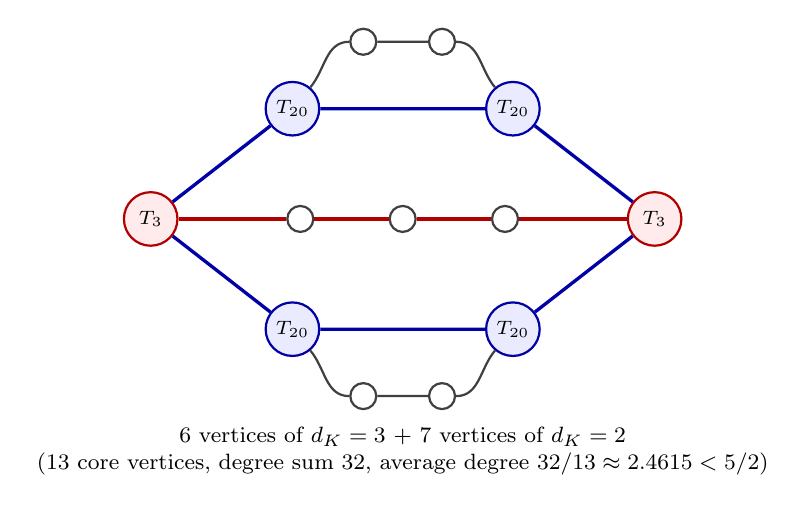
\begin{tikzpicture}[
  t3/.style={circle,draw=red!70!black,fill=red!8,thick,minimum size=6.8mm,inner sep=0.5pt,font=\scriptsize\bfseries},
  t20/.style={circle,draw=blue!65!black,fill=blue!8,thick,minimum size=6.8mm,inner sep=0.5pt,font=\scriptsize\bfseries},
  d2/.style={circle,draw=black!75,fill=white,thick,minimum size=3.3mm,inner sep=0pt},
  edge/.style={thick,black!75}
]
% 6-cycle of coreDeg=3 vertices
\node[t3]  (T1) at (-3.2, 0) {$T_3$};
\node[t3]  (T2) at ( 3.2, 0) {$T_3$};
\node[t20] (A1) at (-1.4, 1.4) {$T_{20}$};
\node[t20] (A2) at ( 1.4, 1.4) {$T_{20}$};
\node[t20] (B1) at (-1.4,-1.4) {$T_{20}$};
\node[t20] (B2) at ( 1.4,-1.4) {$T_{20}$};

% 6-cycle good edges
\draw[edge,blue!65!black,very thick] (T1) -- (A1) -- (A2) -- (T2) -- (B2) -- (B1) -- (T1);

% 3-thread between T1 and T2
\node[d2] (m1) at (-1.3, 0) {};
\node[d2] (m2) at ( 0.0, 0) {};
\node[d2] (m3) at ( 1.3, 0) {};
\draw[edge,red!70!black,very thick] (T1) -- (m1) -- (m2) -- (m3) -- (T2);

% Top 2-thread between A1 and A2
\node[d2] (u1) at (-0.5, 2.25) {};
\node[d2] (u2) at ( 0.5, 2.25) {};
\draw[edge] (A1) to[out=50,in=180] (u1) -- (u2) to[out=0,in=130] (A2);

% Bottom 2-thread between B1 and B2
\node[d2] (d1) at (-0.5,-2.25) {};
\node[d2] (d2n) at ( 0.5,-2.25) {};
\draw[edge] (B1) to[out=-50,in=180] (d1) -- (d2n) to[out=0,in=-130] (B2);

\node[font=\footnotesize,align=center] at (0,-2.95) {$6$ vertices of $d_K=3$ $+$ $7$ vertices of $d_K=2$\\($13$ core vertices, degree sum $32$, average degree $32/13 \approx 2.4615 < 5/2$)};
\end{tikzpicture}
\caption{The $13$-vertex periodic core barrier network of average degree $32/13$ (Proposition~\ref{prop:walls}(b)). Every vertex satisfies all global $\mad < 5/2$ structural rules and all $T_3$ adjacency bans of Theorem~\ref{thm:T3-adj}, while the central $T_3(d_G=4)\text{--}3\text{-thread--}T_3(d_G=4)$ pair is locally list-blocked.}
\label{fig:barrier}
\end{figure}

We emphasize that Propositions~\ref{prop:blocking} and~\ref{prop:walls} constitute obstructions to \emph{bounded-radius local list-extension} rather than global counterexamples to Conjecture~\ref{conj:kappa} (all three periodic networks are easily globally PCF $\kappa_G$-choosable). Advancing beyond $22/9$ toward $\mad(G) < 5/2$ (planar girth $g \ge 10$) appears to require either longer-range chain reductions (breaking the $27$-vertex $22/9$ coupling chain by jointly reducing $T_3 - T_{20} - T_{21}$ clusters) or non-local potential/DP-coloring techniques capable of bypassing the $32/13$ and $52/21$ local barriers.

\bibliographystyle{plain}
\bibliography{references}

\end{document}
